\documentclass[a4paper, 12pt]{article} 
\usepackage{float}
\usepackage{geometry}
\usepackage[new]{old-arrows}
\usepackage{amsthm, amsmath, amssymb}
\usepackage{hyperref}
\usepackage{microtype}
\usepackage{enumitem}
\usepackage{titletoc}
\usepackage{titlesec}
\usepackage{cleveref}
\usepackage{tikz}

\usetikzlibrary{fadings}

\usetikzlibrary{cd}

\newtheorem{thm}{Theorem}[section]
\newtheorem{lemma}[thm]{Lemma}
\newtheorem{fact}[thm]{Fact}
\newtheorem{cor}[thm]{Corollary}
\newtheorem{prop}[thm]{Proposition}
\newtheorem{problem}[thm]{Problem}

\theoremstyle{definition}
\newtheorem{defi}[thm]{Definition}
\newtheorem{notation}[thm]{Notation}
\newtheorem{eg}[thm]{Example}
\newtheorem{remark}[thm]{Remark}

\newcommand\Z{\mathbb{Z}}
\newcommand\N{\mathbb{N}}
\newcommand\Q{\mathbb{Q}}
\newcommand\R{\mathbb{R}}
\renewcommand\d{\mathrm{d}}
\newcommand\GL{\mathrm{GL}}
\newcommand\Wh{\mathrm{Wh}}
\newcommand\Cl{\mathrm{Cl}}
\newcommand\cell{\mathrm{cell}}

\DeclareMathOperator\Hom{Hom}
\DeclareMathOperator\Pic{Pic}
\DeclareMathOperator\im{im}
\DeclareMathOperator*\colim{colim}
\newcommand\fakeqed{\pushQED{\qed}\qedhere}

\tikzset{circ/.style = {fill, circle, inner sep = 0, minimum size = 3}}
\titleformat{\section}{\normalfont\Large\sc}{\thesection}{1em}{}

\makeatletter
\renewcommand\tableofcontents{\@starttoc{toc}}
\makeatother

% evil
\let\LaTeXStandardTableOfContents\tableofcontents
\renewcommand{\tableofcontents}{%
\begingroup%
\renewcommand{\bfseries}{\sc}%
\LaTeXStandardTableOfContents%
\endgroup%
}%

\begin{document}
\hspace{0pt}
\vfill
\begin{center}
  \sc\Huge Geometric Topology\vspace{140pt}
\end{center}
\thispagestyle{empty}
\vfill
\hspace{0pt}
\pagebreak

\begin{center}
  \sc
  {\huge Geometric Topology}\vspace{20pt}\\
  {\Large Easter 2018}
\end{center}
\vspace{40pt}
\begin{center}
  \begin{minipage}{0.8\textwidth}
    \tableofcontents
  \end{minipage}
\end{center}

\thispagestyle{empty}

\setcounter{page}{1}
\pagebreak

\section{Introduction}
The basic idea is that we have some sort of object, and we want to know when it is ``simple''. More precisely, we will try to understand the following problems:
\begin{enumerate}
  \item We have a space and we want it to be a finite CW complex.
  \item We have a cobordism and we want it to be trivial, i.e.\ a product $M \times [0, 1]$.
  \item We have an open manifold and we want it to be the interior of a manifold with boundary.
  \item We have a map $f: M \to S^1$, and we want this to be homotopic to a fiber bundle projection.
\end{enumerate}
Of course, not all objects are ``simple''. What we usually do is to impose some conditions that make the conclusion even plausible. We then see if they are enough. For example, for (1), a possible condition is that the homology groups are finitely generated.

It is often the case that our assumptions are not strong enough, but in subtle ways. When we try to geometrically simplify our object, we will encounter some \emph{obstructions}. These are usually elements in an abelian group that depends on the fundamental group of our space. We then find that we can solve the problem if and only if the obstruction vanishes. A particularly useful case is when the group the obstruction lies in vanishes. In this case, there is always no obstruction, and we win. In the cases we care about, this will be the case if the space is simply connected.

Of course, what obstruction comes up is a function of what assumptions we initially impose on our space. In fact, for the sake of exposition, in (3) and (4), we will impose conditions so strong that no obstruction occurs. Elsewhere in the literature, it is often the case that weaker conditions are imposed, and then there will be interesting obstructions.

\section{Wall's Finiteness Obstruction}
One of the best kinds of spaces to work with is finite CW complexes. Thus, it is natural to ask the question
\begin{problem}
  When is a topological space weak homotopy equivalent to a finite CW complex?
\end{problem}
Applying a CW approximation and  Whitehead's theorem, we can equivalently ask
\begin{problem}
  When is a CW complex homotopy equivalent to a finite CW complex?
\end{problem}

We might try to answer this question using familiar tools from algebraic topology --- necessary conditions include having finitely presented fundamental group and finitely generated homology groups with bounded dimension. But this is not quite enough, since upon a moment of thought, all these conditions are also satisfied by spaces that are retracts of finite CW complexes.

\begin{defi}
  A CW complex is \emph{finitely dominated} if it is a retract of a finite CW complex (in the homotopy category).
\end{defi}
It turns out we can indeed characterize finitely dominated spaces by imposing finiteness conditions on the fundamental group and (co)homology groups \cite[Lecture 1, Proposition 22]{lurie-281}. We are thus led to consider the following problem:

\begin{problem}
  When is a finitely dominated CW complex in fact homotopy equivalent to a finite CW complex?
\end{problem}
In general, this is not always true. By the end of the section, we shall see that the obstruction to this problem lies in a group called the \emph{zeroth Whitehead group} $\Wh_0(\pi_1 X)$, which in particular vanishes when $\pi_1X$ is trivial. So if we restrict to simply connected spaces, the answer is ``always''.

It is possible to approach this problem from a rather geometric point of view, by attempting to exhibit our space $X$ as a finite CW complex, and see what obstructions we encounter. However, the true nature of the obstruction is more easily appreciated if we take an algebraic approach.

The idea is that instead of taking the homology of the singular chain complex $C_*(X)$, which is a rather crude invariant, we consider it as an object of the derived category and try to obtain more nuanced invariants from it.

However, na\"ively, this only retains $H_1$ information, not $\pi_1$, and we just said this is important. The standard way to take $\pi_1$ into account while doing homology is to use homology with local coefficients. This amounts to viewing $X$ as the quotient of its universal cover $\tilde{X}$ by the natural $\pi_1 X$-action, and hence consider $C_*(\tilde{X})$ as a chain complex of $\Z[\pi_1 X]$-modules. We can recover $C_*(X)$ by $C_*(X) = C_*(\tilde{X}) \otimes_{\Z[\pi_1 X]} \Z$.

The fundamental observation is that if $X$ is a finite CW complex, then we have a quasi-isomorphism $C^{\cell}_*(X) \to C_*(X)$, and the source is a finitely generated free abelian group. More generally, the cell structure of $X$ lifts to one of $\tilde{X}$, and then $C^{\cell}_*(\tilde{X})$ of $\tilde{X}$ is a finitely generated free $\Z[\pi_1 X]$-module, quasi-isomorphic to $C_*(\tilde{X})$. Conversely, we will show that if $C_*(\tilde{X})$ is quasi-isomorphic to a complex of finite free $\Z[\pi_1 X]$-modules, then this gives a prescription of how we can build $X$ as a finite CW complex.

How does the finite domination come in? Suppose $X$ is only finitely dominated. By adding finitely many cells to the dominating complex, we may assume the retraction maps induce isomorphisms on $\pi_1$, which allows us to compare their singular chain complexes (or rather, the singular chain complexes of their lifts as $\Z[\pi_1 X]$-modules). We then know that $C_*(\tilde{X})$ is a retract of a finite free chain complex. It is not necessarily the case that $C_*(\tilde{X})$ is quasi-isomorphic a finite free chain complex. Indeed, a retract of a free module is only a projective module. So it might be more reasonable to expect $C_*(\tilde{X})$ to be quasi-isomorphic a finitely generated projective chain complex, and this is indeed true.

\begin{thm}[{\cite[Proposition 3.2]{ranicki}}]
  Let $R$ be a ring, and let $C_*$ be an $R$-chain complex that is a retract of a finite free chain complex $F_*$ in the derived category. Then $C_*$ is quasi-isomorphic to a finitely generated projective chain complex $P_*$. Moreover, if $F_*$ is concentrated in degrees $[a, b]$, then we can pick $P_*$ to be concentrated in $[a, b]$ as well.\fakeqed
\end{thm}
The proof is a (slightly) clever trick that turns the homotopy retraction into a genuine retraction.\footnote{As a rule of thumb, proofs of purely algebraic results will often be omitted. I am, however, ambivalent about the inclusion of this proof. On the one hand, this result is the crux of the whole argument. On the other hand, the proof does not provide any enlightenment. I have settled for exclusion, for the techniques in the proof are orthogonal to the rest of the essay.}

We will see that the failure of a finitely dominated space to be finite is the same as the failure of a projective module to be free. The latter is measured by the $K_0$ group.
\begin{defi}
  Let $R$ be a ring. We define $K_0(R)$ to be the Grothendieck group of finitely generated projective $R$-modules (up to isomorphism), where we impose
  \[
    [M] \oplus [N] = [M \oplus N].
  \]
  We write $\tilde{K}_0(R)$ for the quotient of $K_0(R)$ by the free modules.

  If $R = \Z[G]$ for a group $G$, then we write $\Wh_0(G) = \tilde{K}_0(\Z[G])$.
\end{defi}
\begin{eg}
  By the classification theorem of finitely generated abelian groups, $\Wh_0(\{e\}) = 0$.
\end{eg}
We can generalize this to chain complexes easily:
\begin{notation}
  If $P_*$ is a bounded chain complex of finitely generated projective $R$-modules, we write
  \[
    \chi(P_*) = \sum_{i = -\infty}^\infty (-1)^i [P_i] \in \tilde{K}_0(R).
  \]
\end{notation}

It is an easy exercise in homological algebra to check that
\begin{prop}
  If $P_*$ is acyclic, then $[P_*] = 0$. Hence, by considering mapping cones, $[P_*]$ depends only on the quasi-isomorphism class of $P_*$.\fakeqed
\end{prop}
This allows us to extend the notation $\chi(P_*)$ to any chain complex that is quasi-isomorphic to a finitely generated projective chain complex. We thus define

\begin{defi}
  Let $X$ be a finitely dominated space. Then \emph{Wall's finiteness obstruction} of $X$ is
  \[
    w(X) = \chi(C_*(\tilde{X})) \in \Z[\pi_1 X].
  \]
\end{defi}
If $X$ is in fact a finite CW complex, then the finiteness obstruction certainly vanishes. The converse is true, and the proof is largely bookkeeping.

To do this, we build a finite CW complex $Z$ dimension by dimension. Since retracts of finitely presented groups are finitely presented, we know $\pi_1 X$ is finitely presented. So we can create a finite CW complex $Z$ and a map $f: Z \to X$ that induces an isomorphism on $\pi_1$. Since $\pi_2(X)$ is finitely generated, by adding sufficiently many $2$-cells to $Z$, we may further assume $f$ is surjective on $\pi_2$. In other words, $f$ is a $2$-equivalence.

To extend $f$ to a $k$-equivalence inductively, suppose $f: Z \to X$ is a $(k - 1)$-equivalence. Then the obstruction to it being a $k$-equivalence is
\[
  \pi_k(X, Z) \cong \pi_k(\tilde{X}, \tilde{Z}) \cong H_k(\tilde{X}, \tilde{Z}),
\]
which is finitely generated $\Z[\pi_1 X]$-modules since both $C_*(\tilde{X})$ and $C_*(\tilde{Z})$ are isomorphic to finitely generated chain complexes. Thus, we can add finitely many $k$-cells to kill off $\pi_k(X, Z)$.

Suppose $C_*(\tilde{X})$ is equivalent to an $n$-dimensional finitely generated projective chain complex $P_*$. We can carry the above procedure up to dimension $n - 1$ without worrying much. When we want to finally reach dimension $n$, we have to add cells carefully so as to not introduce a non-zero $\pi_{n + 1}(X, Z)$. This works if and only if $\pi_n(X, Z) \cong H_n(\tilde{X}, \tilde{Z})$ is a free $\pi_1 X$-module, in which case will simply add cells corresponding to a basis.

But this is necessarily (almost) the case. Indeed, if $Q_*$ is a finitely projected projective chain complex whose homology is concentrated in the top degree, then by picking a splitting, it is easy to see that
\[
  \chi(Q_*) = \chi(H_*(Q)).
\]
Since the Euler characteristic is additive on short exact sequences, it follows that
\[
  (-1)^n [H_n(\tilde{X}, \tilde{Z})] = \chi(P_*) - \chi(C_*^{\cell}(Z)) = 0.
\]
So $H_n(\tilde{X}, \tilde{Z})$ is stably free, i.e.\ $H_n(\tilde{X}, \tilde{Z}) \oplus \Z[\pi_1 X]^r$ is free for some $r$. We can then wedge $r$ many $(n-1)$-cells onto $Z$ which map trivially to $X$, when adds a copy of $\Z[\pi_1 X]^r$ to $H_n(\tilde{X}, \tilde{Z})$, thereby making it free. Thus, we conclude
\begin{thm}[Wall, \cite{wall-finiteness}]
  Let $X$ be a finitely dominated space. Then $X$ is a finite CW complex (up to homotopy equivalence) iff $w(X) = 0$.

  Moreover, if $X$ is dominated by a CW complex of dimension $n$ and $w(X) = 0$, then $X$ has the homotopy type of a finite CW complex of dimension $n$.
\end{thm}

\begin{cor}
  If $X$ is a finite CW complex and is dominated by another finite CW complex of dimension $n$, then $X$ has the homotopy type of a finite CW complex of dimension $n$.
\end{cor}

Running the same argument in the relative context shows that
\begin{cor}\label{cor:dim-dom-rel}
  If $(X, A)$ is a finite relative CW complex and is dominated rel $A$ by a finite relative CW complex $(Y, A)$ of dimension $n$ (i.e.\ $Y$ is obtained from $A$ by adding finitely many cells of dimension $\leq n$), then $(X, A)$ is a finite relative CW complex of dimension $n$.
\end{cor}

To ensure the theory is not vacuous, there are two things we should verify:
\begin{enumerate}
  \item There are finitely presented groups $G$ with $\Wh_0(G) \not= 0$.
  \item For each finitely presented group $G$ and $\eta \in \Wh_0(G)$, there is a finitely dominated space $X$ with $\pi_1 X = G$ and $w(X) = \eta$.
\end{enumerate}
We leave the readers to investigate (2) themselves, which is a simple direct construction. On the other hand, (1) is more difficult. We shall discuss a rather special case.

The first observation is that for any \emph{commutative} ring $R$, there is a determinant map
\[
  \det: K_0(R) \to \Pic(R),
\]
sending a projective module to its top exterior power (it may or may not help to think of projective modules as locally free sheaves). This is well-defined because $\det(P \oplus P') = \det P \otimes \det P'$. Moreover, this is surjective, since the determinant of a line bundle is the line bundle itself.

Since the determinant of a free $R$-module is trivial, the determinant map factors through $\tilde{K}_0(R)$. Thus, if we want to show that $\tilde{K}_0(R)$ is non-trivial, it suffices to show that $\Pic(R)$ is non-trivial.

For $\Z[G]$ to be commutative, we must pick $G$ to be an abelian group, and the simplest possible example is $G = C_p$, a cyclic group of prime order. There is a natural map
\[
  \Z[C_p] \to \Z[\zeta_p] = \mathcal{O}_{\Q[\zeta_p]},
\]
sending the generator $g$ to $\zeta_p$. This has kernel generated by $1 + g + \cdots + g^{p - 1}$.

It was shown by Rim \cite[Theorem 6.24]{modules-over-finite-groups} that this induces an isomorphism on $\tilde{K}_0$. In fact, the determinant map is an isomorphism \cite[Theorem 6.19]{modules-over-finite-groups}. So we are left with the problem of computing the class group of $\Q[\zeta_p]$.

This is a problem better left for a number theorist to solve. I shall merely report on their discoveries.
\begin{thm}
  $\Cl(\Q[\zeta_p])$ vanishes for $p < 23$, but is non-zero for $p = 23$.\fakeqed
\end{thm}
See \url{https://oeis.org/A055513} for a detailed list and some references, and \cite{washington-cyclotomic-fields} for general theory.

\section{The Whitehead torsion}
We now know when a CW complex is homotopy equivalent to a finite CW complex. Now suppose we have two finite CW complexes $X, Y$, and a homotopy equivalence $f: X \to Y$ between them. Can we ``construct'' this homotopy equivalence in finitely many ``steps''? To be precise, we want to allow for the following two operations:
\begin{enumerate}
  \item We can replace $X$ with $X \vee D^k$, or vice versa.
  \item We can ``slide'' the attaching map of an $n$-cell along another $n$-cell:
    \begin{figure}[H]
      \centering
      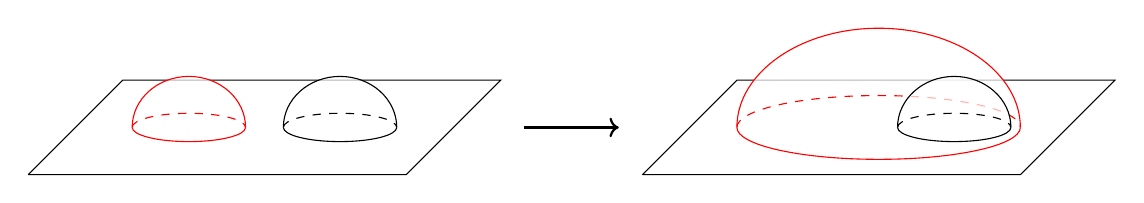
\begin{tikzpicture}[scale=1.2]
        \draw (0, 0) -- (4, 0) -- (5, 1) -- (1, 1) -- (0, 0);

        \begin{scope}[shift={(3.3, 0.5)}, scale=0.3]
          \draw [fill=white, fill opacity=0.7] (-2, 0) arc (180:0:2 and 1.8);
          \draw (-2, 0) arc (180:360:2 and 0.5);
          \draw [dashed] (-2, 0) arc (180:0:2 and 0.5);
        \end{scope}

        \begin{scope}[shift={(1.7, 0.5)}, scale=0.3]
          \draw [red, fill=white, fill opacity=0.7] (-2, 0) arc (180:0:2 and 1.8);
          \draw [red] (-2, 0) arc (180:360:2 and 0.5);
          \draw [dashed, red] (-2, 0) arc (180:0:2 and 0.5);
        \end{scope}

        \draw [->, thick] (5.25, 0.5) -- (6.25, 0.5);

        \begin{scope}[shift={(6.5, 0)}]
          \draw (0, 0) -- (4, 0) -- (5, 1) -- (1, 1) -- (0, 0);

          \begin{scope}[shift={(2.5, 0.5)}, scale=0.75]
            \draw [red, fill=white, fill opacity=0.7] (-2, 0) arc (180:0:2 and 1.4);
            \draw [red] (-2, 0) arc (180:360:2 and 0.45);
            \draw [dashed, red] (-2, 0) arc (180:0:2 and 0.45);
          \end{scope}

          \begin{scope}[shift={(3.3, 0.5)}, scale=0.3]
            \draw [fill=white, fill opacity=0.7] (-2, 0) arc (180:0:2 and 1.8);
            \draw (-2, 0) arc (180:360:2 and 0.5);
            \draw [dashed] (-2, 0) arc (180:0:2 and 0.5);
          \end{scope}
        \end{scope}
     \end{tikzpicture}
    \end{figure}
\end{enumerate}

We then say a homotopy equivalence $f: X \to Y$ is ``simple'' if it is given by performing finitely many of the above steps to $X$. We shall, as before, come up with an algebraic obstruction to the simplicity of a homotopy equivalence. We will not show (but it is true, see \cite[Chapter 13]{whitehead-torsion-source}) that a homotopy equivalence is simple in this sense if the obstruction vanishes. Instead, we define a homotopy equivalence to be simple if the obstruction vanishes, which is all we need for the $s$-cobordism theorem.

Algebraically, a CW structure on $X$ gives us a free $\pi_1X$-chain complex quasi-isomorphic to $C_*(\tilde{X})$. This almost comes with a preferred choice of basis, except that there is not a unique lift of the cell to the universal cover, and the ordering of the cells is not canonically defined.

Putting these issues aside, we from now on assume our chain complexes are all finite and comprised of free $R$-modules (for a fixed ring $R$) with a preferred choice of basis. We are then led to looking at when a homotopy equivalence of such chain complexes is simple. Equivalently, passing to the mapping cone, when a contractible chain complex is ``simply contractible''. On the level of chain complexes, the two operations above correspond to
\begin{enumerate}
  \item Adding $R$ to degrees $q$ and $q + 1$ and taking the identity map on them.
  \item Performing column operations on the differentials.
\end{enumerate}
A bit more should be said about (2). Performing column operations is the same as changing the basis of the source. Thus, if we have a sequence $A \overset{f}{\to} B \overset{g}{\to} C$ and we perform column operations on $g$, then we must perform analogous row operations on $f$ if we want it to remain a complex. Geometrically, this is the observation that if we slide the attaching map of an $n$-cell over another $n$-cell, then we must modify the attaching map of the $n+1$-cells accordingly. At the end, we will focus on chain complexes concentrated in two adjacent degrees, so (2) becomes ``Perform row and column operations on the differentials''.

The first observation is that with operations (1) and (2), we can replace our chain complex with one concentrated in two degrees only. Suppose our chain complex ends like
\[
  \begin{tikzcd}
    A \ar[r, "f"] & B \ar[r, "g"] & C \ar[r] & 0
  \end{tikzcd}
\]
Since $C$ is free, we can use (1) to add copies of $C$ to the positions of $A$ and $B$:
\[
  \begin{tikzcd}
    A \oplus C \ar[r, "f \oplus 1_C"] & B \oplus C \ar[r, "g\oplus 0"] & C \ar[r] & 0
  \end{tikzcd}
\]
Now since our complex was acyclic, there is a chain contraction, which in the lowest degree means a section $s$ of $g$. This section instructs us how we can perform column operations on $g \oplus 0$ to turn it into $g \oplus 1_C$, and a bit of linear algebra exercise shows that the corresponding row operations on $f \oplus 1$ will leave us with
\[
  \begin{tikzcd}
    A \oplus C \ar[r, "f \oplus s"] & B \oplus C \ar[r, "g\oplus 1_C"] & C \ar[r] & 0.
  \end{tikzcd}
\]
We can now perform (1) again to end up with
\[
  \begin{tikzcd}
    A \oplus C \ar[r, "f \oplus s"] & B \ar[r] & 0 \ar[r] & 0.
  \end{tikzcd}
\]
While $s$ is not well-defined, it is well-defined up to an element in the kernel of $g$, i.e.\ an element in the image of $f$. So $f \oplus s$ is well-defined up to a column operation.

By iterating this, we are left with a chain complex concentrated in two adjacent degrees, and the differential is a single $N \times N$ matrix.
\begin{defi}
  Let $R$ be a ring. We define
  \[
    \GL(R) = \colim_{n \to \infty} \GL_n(R),
  \]
  where the inclusion $\GL_n(R) \to \GL_{n + 1}(R)$ is given by
  \[
    A \mapsto 
    \begin{pmatrix}
      A & 0\\
      0 & 1
    \end{pmatrix}.
  \]
  We then define $K_1(R)$ to be the quotient of $\GL_n(R)$ by the subgroup generated by elementary row and column operations.
\end{defi}
Then a matrix with coefficients in $R$ up to the operations defined in (1) and (2) is exactly an element of $K_1(R)$.

In fact, the subgroup generated by row and column operations is a normal subgroup, and turns out to be $[\GL(R), \GL(R)]$. So $K_1(R)$ is an abelian group. To show this, one simply writes out explicit formulas for commutators in terms of row and column operations and vice versa, which is done in \cite{milnor-whitehead-torsion}.

By more linear algebra exercise, we can describe the result of iterating the above procedure as
\begin{defi}
  Let $(C_*, d_*)$ be a acyclic chain complex, and let $c_*$ be a contraction. Write $C_{\mathrm{odd}}$ and $C_{\mathrm{even}}$ for the direct sums of the odd and even parts respectively with the inherited basis. We define the \emph{Whitehead torsion} $\tau(C_*) \in K_1(R)$ to be the class of the matrix of $d_* + c_*$.

  If $f: C_* \to D_*$ is a quasi-isomorphism of chain complexes, the Whitehead torsion $\tau(f)$ is defined to be the Whitehead torsion of the mapping cone.
\end{defi}
The fact that this doesn't depend on the choice of $c_*$ follows from the fact that the procedure described previously is well-defined up to column operations. One can also prove this directly, disregarding the previous discussion completely, which is again done in \cite{milnor-whitehead-torsion}.

An honest mathematician would carefully explain how we should order the basis when we define $C_{\mathrm{odd}}$ and $C_{\mathrm{even}}$ (and the mapping cone), or else the result will be defined only up to a sign. However, in our geometric application, there is no ordering of the basis in the first place, and instead, we consider
\begin{defi}
  If $G$ is a group, we define the Whitehead group to be
  \[
    \Wh(G) = \Wh_1(G) = K_1(\Z[G])/\{\pm g: g \in G\}.
  \]
\end{defi}
We can then unambiguously define
\begin{defi}
  If $f: X \to Y$ is a homotopy equivalence of finite CW complexes, then the \emph{Whitehead torsion} $w(f) \in \Wh(\pi_1X)$ is defined to be the Whitehead torsion of $f_*: C^{\cell}_*(\tilde{X}) \to C^{\cell}_*(\tilde{Y})$, where the bases are given by any lift of the cells of $X$ and $Y$ respectively. Note that a cellular approximation has to be chosen, and (the mapping cone of) $f_*$ will be well-defined up to column operations.

  A homotopy equivalence with trivial Whitehead torsion is said to be a \emph{simple homotopy equivalence}.
\end{defi}

Again to show our theory is non-vacuous, we need to show that $\Wh(G)$ is not always zero. Observe that the determinant map $\det: K_1(G) \to \Z[G]^\times$ induces a natural surjection
\[
  \det: \Wh(G) \twoheadrightarrow (\Z[G])^\times/\{\pm g\}.
\]
Thus, it suffices to show that $(\Z[G])^\times/\{\pm g\}$ is not always zero.
\begin{eg}
  Let $t$ be the generator of $C_5$. Then in $\Z[C_5]$, we have the identity
  \[
    (t + t^{-1} - 1)(t^2 + t^{-2} - 1) = 1.
  \]
  Thus, $t + t^{-1} - 1$ is a non-trivial unit, and $\Wh(C_5)$ is non-trivial.
\end{eg}
On the other hand, an important result is
\begin{eg}
  By the Smith normal form theorem, $\Wh(\{e\}) = 0$.
\end{eg}

The existence of finitely dominated CW complexes with prescribed Whitehead torsion will be discussed when we talk about the $s$-cobordism theorem. Instead, we have a more serious problem to address.

The definition of the Whitehead torsion depends crucially on the CW structure on our topological space. It is true that the Whitehead torsion is a topological invariant. Equivalently, every homeomorphism is a simple homotopy equivalence. This is a hard theorem by Chapman \cite{chapman-topological-invariance}. For our purposes, we will need the following very specific result:
\begin{thm}
  Let $W$ be an $h$-cobordism between $M$ and $N$, i.e.\ a cobordism where the inclusions $\iota: M \hookrightarrow W$ and $\iota': N \hookrightarrow W$ are homotopy equivalences. Then $w(\iota)$ is well-defined if we pick a CW structure induced by a Morse function.
\end{thm}

\begin{proof}[Proof sketch]
  First observe that subdividing any of the cells in the CW structure does not change the Whitehead torsion. By performing such subdivisions, one can show that the CW structure given by a Morse function is equivalent (for the purposes of Whitehead torsion) to that given by a smooth triangulation, i.e.\ a triangulation where the inclusion of each simplex is a smooth map.

  It is a theorem of Whitehead that after subdivision, any two smooth triangulations are isomorphic. Note that this is not the same as saying they have a common refinement. Instead, if $(K_i, L_i)$ are (subdivisions of) the triangulations exhibited by maps $\phi_i: (K_i, L_i) \to (M, W)$, then there is an isomorphism of abstract simplicial complexes $\psi: (K_1, L_1) \to (K_2, L_2)$, which need not respect $\phi_i$. Then the Whitehead torsion induced by the two triangulations differ by an action of $(\phi_2 \circ \psi \circ \phi_1^{-1})_* : \Wh(\pi_1W) \to \Wh(\pi_1W)$. As part of the statement of Whitehead's theorem, we can make $\phi_2 \circ \psi \circ \phi_1^{-1}$ as close to the identity as possible, and in particular we can choose it to act as the identity on $\pi_1$. So $(\phi_2 \circ \psi \circ \phi_1^{-1})_*$ is also the identity, and hence the Whitehead torsion is well-defined.
\end{proof}
See \cite{milnor-whitehead-torsion} for a slightly less sketchy proof.

\section{The \texorpdfstring{$s$}{s}-cobordism theorem}\label{sec:s-cobordism}
We are now ready to tackle the $s$-cobordism theorem. Suppose we are given an $h$-cobordism $(W, M, N)$. When is this trivial? In other words, when is there an isomorphism $W \cong M \times [0, 1]$? In 1962, Smale \cite{smale-h-cobordism} showed that this is always the case if $M$ is simply connected. On the other hand, since $M \times [0, 1]$ can be obtained from $M$ by replacing each $n$ cell $D^n$ with $D^n \times D^1$, one sees that $\tau(W, M) = \tau(\iota: M \hookrightarrow W) = 0$ is a necessary condition for $W$ to be trivial. In fact, this is sufficient.

\begin{thm}[$s$-cobordism theorem, \cite{mazur-s-cobordism} \cite{stallings-s-cobordism}]
  Let $(W, M, N)$ be an $h$-cobordism of dimension $n \geq 6$. Then $W$ is trivial if and only if the Whitehead torsion $\tau(W, M) = 0$.
\end{thm}
The proof we present is adapted from \cite{luck-surgery}.

\begin{remark}
  We defined an $h$-cobordism to be one where $M, N \hookrightarrow W$ are homotopy equivalences. In practice, Lefschetz duality implies it suffices to check that one of the inclusions is a homotopy equivalence, and both maps induce isomorphisms on $\pi_1$.
\end{remark}

Before we begin to prove the theorem, we state two standards result from differential topology that we will use frequently. See, for example Chapter 6 of \cite{lee-smooth-manifolds} (he only proves a special case of the second theorem, but the same proof applies).
\begin{thm}
  Let $f: M \to N$ be a continuous map between manifolds, smooth on a closed subset $A \subseteq M$. Then $f$ is homotopic rel $A$ to a smooth map. 
\end{thm}

\begin{thm}
  Let $f: M \to N$ be a smooth map between manifolds which is an embedding on a closed subset $A \subseteq M$. If $\dim N \geq 2 \dim M + 1$, then $f$ is homotopic rel $A$ to a smooth embedding.
\end{thm}

The idea is to show that every simplification move allowed in the definition of the Whitehead group can be geometrically realized in our manifold. Since each of those moves had a geometric motivation, we might expect this to be straightforward, but there are two subtleties:
\begin{itemize}
  \item In our original motivation, we worked with CW complexes, but here we need to take care of the smooth structure.
  \item In homology, there can be cancellation, i.e.\ if my attaching map winds around a loop $\gamma$ once, does something else, and then winds around $\gamma$ in the opposite direction, then these two contributions cancel in homology, but not necessarily geometrically. We thus need to be able to eliminate things geometrically when there is cancellation in homology.
\end{itemize}
The first problem will be addressed by the theory of handlebody decompositions, and the second by Whitney's trick. We will get to Whitney's trick when we need it, and instead start by discussing handlebody decompositions.

\begin{defi}
  An $n$-dimensional handle of index $q$ is $D^q \times D^{n - q}$. If $M$ is a manifold and $\phi^q: S^{q - 1} \times D^{n - q} \to \partial_1 W$ is an embedding, then we define
  \[
    M + (\phi^q) = M \cup_{\phi^q} D^q \times D^{n - q}.
  \]
  We will use $(\phi^q)$ to refer to the handle itself, while $\phi^q$ is the attaching map. We adopt the following terminology:
  \begin{itemize}
    \item The \emph{core} is $D^q \times \{0\}$.
    \item The \emph{transverse sphere} is $\{0\} \times S^{n - q - 1}$.
  \end{itemize}
\end{defi}

\begin{figure}[H]
  \centering
  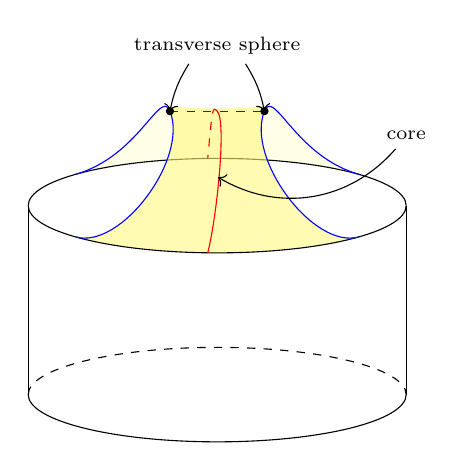
\begin{tikzpicture}[scale=1.2]
    \fill [yellow!50!white, opacity=0.2] (-1.5, 2.331) .. controls +( 15.83:0.7) and (-0.6, 3.25) .. (-0.5, 3) to [bend right=25] (-0.55, 3.055) to [bend right=5] (0.55, 3.055) to [bend right=25] (0.5, 3) .. controls (0.6, 3.25) and (0.8265, 2.522) .. (1.5, 2.331) arc(41.4:138.6:2 and 0.5);

    \draw [dashed] (-2, 0) arc(180:0:2 and 0.5);
    \draw (-2, 0) arc(180:360:2 and 0.5);

    \draw (-2, 0) -- (-2, 2);
    \draw (2, 0) -- (2, 2);

    \draw (-2, 2) arc(180:0:2 and 0.5);

    \fill [yellow!50!white, opacity=0.6] (-1.5, 1.669) .. controls +(-15.83:0.5) and (-0.3, 2.5) .. (-0.5, 3) to [bend right=25] (-0.55, 3.055) to [bend right=5] (0.55, 3.055) to [bend right=25] (0.5, 3) .. controls (0.3, 2.5) and (1.019, 1.533) .. (1.5, 1.669) arc(318.6:221.4:2 and 0.5);


%      \fill [blue, opacity=0.4] (2, 2) arc(0:-41.4:2 and 0.5) .. controls +(195.83:0.5) and (0.3, 2.5) .. (0.5, 3) to [bend left=25] (0.55, 3.055) .. controls (1.3, 3.055) and (2, 3) .. (2, 2);
    \draw (-2, 2) arc(180:360:2 and 0.5);
    \foreach \r in {1, -1} {
      \begin{scope}[xscale=\r]
%        \fill [white] (-1.5, 1.669) .. controls +(-15.83:0.5) and (-0.3, 2.5) .. (-0.5, 3) -- (0.5, 3);
        \draw [blue] (-1.5, 1.669) .. controls +(-15.83:0.5) and (-0.3, 2.5) .. (-0.5, 3);
        \draw [blue] (-1.5, 2.331) .. controls +( 15.83:0.7) and (-0.6, 3.25) .. (-0.5, 3);
      \end{scope}
    }
%    \fill[white] (-0.45, 2.4) rectangle (0.45, 2.6);

    \draw [green!30!black, dashed] (-0.5, 3) -- (0.5, 3);
    \draw [red](-0.1, 1.5) .. controls (0, 1.9) and (0.1, 2.9) .. (0, 3);
    \draw [dashed, red] (0, 3) .. controls (-0.05, 3.05) .. (-0.1, 2.5);

    \node [circ] at (0.5, 3) {};
    \node [circ] at (-0.5, 3) {};
    \draw (0.3, 3.5) edge [bend left=10, ->] (0.5, 3);
    \draw (-0.3, 3.5) edge [bend right=10, ->] (-0.5, 3);
    \node [above] at (0, 3.5) {\scriptsize transverse sphere};

    \draw (2, 2.6) node [above] {\scriptsize core} edge [bend left=40, ->] (0.01, 2.3);


  \end{tikzpicture}
  \caption{An example of a $1$-handle for $n = 2$}
\end{figure}
It is a standard result in Morse theory that given a cobordism $W$ between $\partial_0 W$ and $\partial_1 W$, we can always find a \emph{handlebody decomposition}
\[
  W = \partial_0 W \times [0, 1] + (\phi_1^{q_1}) + \cdots + (\phi_r^{q_r}).
\]
In this section, all isomorphisms are required to fix $\partial_0 W$.

From a purely homotopy theoretic point of view, adding a $q$-handle is the same as adding a $q$-cell by retracting to the core. Thus, a handlebody decomposition simultaneously gives rise to a CW structure, and the intersection between the attaching map and the transverse sphere encodes the differentials in the CW structure. To actually get the skeletal filtration, it is convenient to arrange our handles in increasing order of index.

First observe that if we have two isotopic attaching maps, then standard differential topology results imply there is a diffeomorphism of $W$ that sends one of the attaching maps to the other. So we know
\begin{lemma}[Isotopy lemma]
  The diffeomorphism type of $W + (\psi^q)$ depends only on the isotopy class of $\psi^q$.\fakeqed
\end{lemma}

Consequently, we get
\begin{lemma}[Commutativity lemma]
  Let $W$ be a cobordism, and $q \leq r$. If
  \[
    V = W + (\psi^r) + (\phi^q),
  \]
  then there is some $\bar{\phi}^q$ such that
  \[
    V \cong W + (\bar{\phi}^q) + (\psi^r).
  \]
\end{lemma}

\begin{proof}
  For dimensional reasons, transversality allows us to isotope $\phi^q$ so that the attaching map does not intersect the transverse sphere of $(\psi^r)$. We then flow $\phi^q$ down along the handle to not intersect $(\psi^r)$ at all.
\end{proof}

We can now write our handlebody decomposition of a cobordism $W$ as
\[
  W = \partial_0 W \times [0, 1] + \sum_{i = 1}^{p_0} (\phi_i^0) + \sum_{i = 1}^{p_1} (\phi_i^1) + \cdots + \sum_{i = 1}^{p_n} (\phi_i^n).
\]
We then have a corresponding cell structure with each $(\phi_i^q)$ corresponding to a $q$-cell, and using local degrees, we see that in the cellular chain complex, the number of copies of $(\phi_i^q)$ in $\mathrm{d} (\phi_j^{q + 1})$ is the number of times $\phi_j^{q + 1}$ hits the transverse sphere of $(\phi_i^q)$, counted with orientation.

The corresponding filtration of $W$ is given by
\begin{align*}
  W_q &= \partial_0 W \times [0, 1] + \sum_{i = 1}^{p_0} (\phi_i^0) + \sum_{i = 1}^{p_1} (\phi_i^1) + \cdots + \sum_{i = 1}^{p_q} (\phi_i^q)\\
  \partial_1 W_q &= \partial W_q - \partial_0 W \times \{0\}\\
  \partial_1^\circ W_q &= \partial_1 W_q - \coprod_{i = 1}^{p_{q + 1}} \phi_i^q(S^q \times \mathrm{int}(D^{n - 1 - q})).
\end{align*}
The last definition is useful if we want to do things without risking messing up our $(q + 1)$-handles.

We can now begin our program to geometrically realize the algebraic operations we previously discussed. Our ultimate goal is to modify the handlebodies so that there are no handlebodies left at the end. For this to be possible at all, we need to be able to perform the operation
\[
  \begin{pmatrix}
    A & 0\\
    * & 1
  \end{pmatrix} \rightsquigarrow A.
\]
This is given by the cancellation lemma:
\begin{lemma}[Cancellation lemma]
  Let $W$ be a cobordism, and suppose we attach a $q$-handle $(\phi^q)$ and then a $q + 1$-handle $(\psi^{q + 1})$ to $W$. If $\psi^{q + 1}(S^q \times \{0\})$ is transverse to the transverse sphere of $(\phi^q)$ and they intersect at exactly one point, then there is a diffeomorphism from $W$ to $W + (\phi^q) + (\psi^{q + 1})$ fixing $\partial_0 W$.
\end{lemma}
We call $(\phi^q), (\psi^{q + 1})$ a cancellation pair.

In a sense, the lemma is self-evident. We will argue that this is indeed the case in two steps --- we first describe a ``standard model'' of a cancellation pair, where it is self-evident that the conclusion holds. It is then also self-evident that any cancellation pair must be equivalent to the standard model in an appropriate sense. 
\begin{eg}
  The picture one should keep in mind is the following:
  \begin{figure}[H]
    \centering
    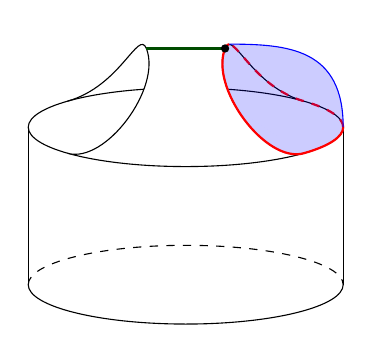
\begin{tikzpicture}
      \draw [dashed] (-2, 0) arc(180:0:2 and 0.5);
      \draw (-2, 0) arc(180:360:2 and 0.5);

      \draw (-2, 0) -- (-2, 2);
      \draw (2, 0) -- (2, 2);

      \draw (0, 2) ellipse (2 and 0.5);

      \foreach \r in {1, -1} {
        \begin{scope}[xscale=\r]
          \fill [white] (-1.5, 1.669) .. controls +(-15.83:0.5) and (-0.3, 2.5) .. (-0.5, 3) -- (0.5, 3);
          \draw (-1.5, 1.669) .. controls +(-15.83:0.5) and (-0.3, 2.5) .. (-0.5, 3);
          \draw (-1.5, 2.331) .. controls +( 15.83:0.7) and (-0.6, 3.25) .. (-0.5, 3);
        \end{scope}
      }
      \fill[white] (-0.45, 2.4) rectangle (0.45, 2.6);

      \draw [green!30!black, thick] (-0.5, 3) -- (0.5, 3);

      \draw [red, thick, dashed] (2, 2) arc(0:41.4:2 and 0.5) .. controls +(164.17:0.7) and (0.6, 3.25) .. (0.5, 3);
      \draw [blue] (0.55, 3.055) .. controls (1.3, 3.055) and (2, 3) .. (2, 2);
      \fill [blue, opacity=0.2] (2, 2) arc(0:-41.4:2 and 0.5) .. controls +(195.83:0.5) and (0.3, 2.5) .. (0.5, 3) to [bend left=25] (0.55, 3.055) .. controls (1.3, 3.055) and (2, 3) .. (2, 2);

      \draw [red, thick] (2, 2) arc(0:-41.4:2 and 0.5) .. controls +(195.83:0.5) and (0.3, 2.5) .. (0.5, 3) edge [bend left=25] (0.55, 3.055);
      \node [circ] at (0.5, 3) {};
    \end{tikzpicture}
    \caption{A $2$-handle cancelling a $1$-handle}
  \end{figure}
  The reader is also encouraged to draw a picture of a $1$-handle cancelling a $0$-handle themselves.

  To put these in words, we write $S^q_{\pm}$ for the northern and southern hemispheres of $S^q$ respectively. Suppose we are given an embedding
  \[
    \mu: S^{q - 1} \times D^{n - q} \cup_{S^{q - 1} \times S^{n - 1 - q}_+} S^q_- \times D^{n - 1 - q} \to \partial_1 W,
  \]
  where we fix an identification of $S^{n - 1 - q}_+$ with $D^{n - 1 - q}$, and $S^{q - 1}$ with $\partial S^q_-$. We can use this to attach a $q$ handle to $\partial_1 W$ via $\phi^q = \mu|_{S^{q - 1} \times D^{n - q}}$. We then attach a $(q + 1)$-handle by defining two functions
  \[
    \psi^{q + 1}_{\pm}: S_{\pm}^q \times D^{n - 1 - q} \to \partial_1(W + (\phi^q))
  \]
  separately that agree on the intersection, and glue them to give a $\psi^{q + 1}$.
  
  We simply let $\psi^{q + 1}_- = \mu|_{S^q_+ \times D^{n - 1 - q}}$, and we define $\psi_+^{q + 1}$ to be the inclusion
  \[
    S^q_+ \times D^{n - q - 1} \cong D^q \times S_+^{n - q - 1} \hookrightarrow D^q \times S^{n - q - 1} = \partial (\phi^q) \subseteq \partial_1(W + (\phi^q)).
  \]
  One then sees that $W + (\phi^q) + (\psi^{q + 1})$ is diffeomorphic to $W$.
\end{eg}

In general, the reason a cancellation pair fails to look like the standard model is that $\psi|_{S^q \times \{0\}}$ can behave in completely crazy ways outside of an infinitesimal neighbourhood of the transverse sphere, and there is no control of what $\psi$ does outside of the $S^q \times \{0\}$ at all. All we know is that infinitesimally, near the transverse sphere and $S^q \times \{0\}$, everything is extremely well-behaved. Thus, what we have to do is to push all the badness far away enough.

\begin{proof}[Proof of lemma]
  By transversality and the implicit function theorem, we can isotope $\psi$ so that in a small neighbourhood $U$ of the transverse sphere, the image of $\psi|_{S^q \times \{0\}}$ looks like
  \begin{center}
    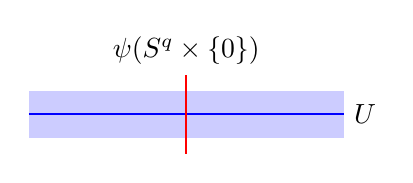
\begin{tikzpicture}
      \fill [opacity=0.2, blue] (-2, -0.3) rectangle (2, 0.3);
      \draw [thick, blue] (-2, 0) -- (2, 0) node [right, black] {$U$};
      \draw [thick, red] (0, -0.5) -- (0, 0.5) node [above, black] {$\psi(S^q \times \{0\})$};
    \end{tikzpicture}
  \end{center}
  Note that this picture is in the \emph{standard} coordinate chart of $(\phi^q) = D^q \times D^{n - q}$, which is a stronger statement than ``there is a coordinate chart where the intersection looks like this''.

  We can further isotope $\psi$, fixing $\psi|_{S^q \times \{0\}}$, so that in a small neighbourhood of $S^q \times \{0\}$, the image looks like
  \begin{center}
    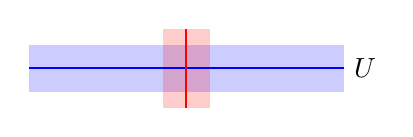
\begin{tikzpicture}
      \fill [opacity=0.2, blue] (-2, -0.3) rectangle (2, 0.3);
      \fill [opacity=0.2, red] (-0.3, -0.5) rectangle (0.3, 0.5);
      \draw [thick, blue] (-2, 0) -- (2, 0) node [right, black] {$U$};
      \draw [thick, red] (0, -0.5) -- (0, 0.5);
    \end{tikzpicture}
  \end{center}
  But we can shrink $S^q \times D^{n - q}$ radially in the $D^{n - q}$ direction so that the image of $\psi$ is exactly this.

  Now apply a flow on $\partial_1 (W + (\phi^q))$ that sends everything in $\partial (\phi^q) \setminus U$ to something outside of $(\phi^q)$, and expands $U$ ``linearly'' to all of $\partial (\phi^q)$. Then this looks exactly like the standard model.
\end{proof}

The natural progression would be to prove that we can perform column operations. However, to talk about such deeds, we ought to take the universal cover of $W$ and work with homology with local coefficients. Thus, it would be nice if our handles don't change the homotopy type of $W$. In other words, if we have no $0$- or $1$-handles.

This will be achieved by replacing $q$-handles with $(q + 2)$-handles, as we did in the algebraic case. If we have a $q$-handle that we want to get rid of, the strategy is to introduce a pair of $(q + 1)$ and $(q + 2)$ handles that cancel each other, such that the $q$-handle and $(q + 1)$-handles also cancel each other.

We need to do this in two steps. First we find a $(q + 1)$-handle that kills the $q$-handle, and then a $(q + 2)$-handles that kill the $(q + 1)$-handle. This is not always possible. For example, if the $q$-handle is responsible for killing off a homology class in degree $q - 1$, and there is no other $q$-handle that can do the job, then it is impossible to add a $(q + 1)$-handle to eliminate the $q$-handle.

Fortunately, if the attaching map of our $q$-handle is null-homotopic, then we would not meet this obstruction. Geometrically, we would want a stronger condition, which adds the word ``embedding'' to the above condition.
\begin{defi}
  We say an embedding $\phi^q: S^{q - 1} \times D^{n - q} \hookrightarrow \partial_1 W$ is trivial if it extends to an embedding $D^q \times D^{n - q} \hookrightarrow \partial_1 W$.

  If we have an embedding $S^{q - 1} \hookrightarrow \partial_1 W$, we say it is trivial if we can extend it to a trivial embedding $S^{q - 1} \times D^{n - q}\hookrightarrow \partial_1 W$.
\end{defi}

It is immediate from the cancellation lemma that
\begin{lemma}
  If $\phi^q$ is a trivial embedding, then we can add a $(q + 1)$-handle $\psi^{q + 1}$ to $W + (\phi^q)$ such that $W \cong W + (\phi^q) + (\psi^{q + 1})$ relative $\partial_0 W$.\fakeqed
\end{lemma}

Now to find a $(q + 2)$-handle that kills off the $(q + 1)$-handle, we have the problem that if the $(q + 1)$-handle $(\phi^{q + 1})$ is responsible for killing off the $q$-handle, then it should be problematic if we want a $(q + 2)$-handle to kill off the $(q + 1)$-handle. What we need is that there is some other existing $(q + 1)$-handle $(\psi^{(q + 1)})$ that kills the $q$-handle (or maybe multiple of them), so that in the presence of $(\psi^{q + 1})$, the attachment map of $(\phi^{q + 1})$ is now trivial.
\begin{lemma}[Elimination lemma]
  Suppose $1 \leq q \leq n - 3$, and that
  \[
    W = \partial_0 W \times [0, 1] + \sum_{i = 0}^{p_q} (\phi_i^q) + \sum_{i = 0}^{p_{q + 1}} (\phi_i^{q + 1}) + \cdots + \sum_{i = 0}^{p_n} (\phi_i^n).
  \]
  Suppose there is a $1 \leq j \leq p_q$ and an embedding $\psi^{q + 1}: S^q \times D^{n - 1 - q}\hookrightarrow \partial_1^\circ W_q$ such that
  \begin{enumerate}
    \item $\psi^{q + 1}|_{S^q \times \{0\}}$ is isotopic in $\partial_1 W_q$ to an embedding $\psi_1^{q + 1}$ that intersects the transverse sphere of $(\phi_j^q)$ at one point transversely, and is disjoint from the transverse spheres of the other $q$-handles.
    \item $\psi^{q + 1}|_{S^q \times \{0\}}$ is isotopic in $\partial_1 W_{q + 1}$ to a trivial embedding $\psi_2^{q + 1}$.
  \end{enumerate}
  Then $W$ is diffeomorphic relative $\partial_0 W$ to a cobordism of the form
  \[
    \partial_0 W \times [0, 1] + \sum_{i \not= j} (\phi_i^q) + \sum_{i = 1}^{p_{q + 1}} (\bar{\phi}_i^{q + 1}) + (\psi^{q + 2}) + \sum_{i = 1}^{p_{q + 2}} (\bar{\phi}_i^{q + 2}) + \cdots + \sum_{i = 1}^{p_n}(\bar{\phi}_i^n).
  \]
\end{lemma}
Note that the condition that $\psi^{q + 1}$ maps into $\partial_1^\circ W_q$ instead of just $\partial_1 W_q$ is not very important. It is needed only so that the condition (2) makes sense.

\begin{proof}
  We may extend $\psi_i^{q + 1}$ and the isotopies to be defined on $S^q \times D^{n - q - 1}$ (we need a framing on the normal bundle, but we can carry that along the isotopies). We may also assume that there are no handles of index $\geq q + 2$, since we can add them back after we are done with this business.
  
  By the previous lemma, there is some $\psi^{q + 2}$ such that $W \cong W + (\psi_2^{q + 1}) + (\psi^{q + 2})$. But by the isotopy lemma, this is diffeomorphic to what we get if we attach $(\psi_1^{q + 1})$ instead of $(\psi_2^{q + 1})$, which by the cancellation lemma, is diffeomorphic to what we get if we didn't have $(\phi_j^q) + (\psi_1^{q + 1})$.
\end{proof}

With the elimination lemma, we can now prove
\begin{lemma}
  Let $W$ be an $n$-dimensional cobordism with $n \geq 6$. If the inclusion $\partial_0 W \hookrightarrow W$ is $1$-connected, then there is a handlebody decomposition of $W$ with no $0$ or $1$ handles.
\end{lemma}
%The converse is, of course, true. 
\begin{proof}
  We pick an arbitrary handlebody decomposition, and use the cancellation and elimination lemmas to get rid of the $0$ and $1$ handles.
  \begin{itemize}
    \item To eliminate the $0$-handles, we apply the cancellation lemma directly. Since every $0$-handle introduces a new connected component, if there is a $0$-handle, then there must be a $1$-handle $(\psi^1)$ that connects the $0$-handle $(\phi^0)$ to $\partial_0 W \times [0, 1]$. The boundary of the core of $(\psi^1)$ is just two points, and there must be exactly one of them on the boundary of $(\phi^0)$, which is also its transverse sphere. So the conditions of the cancellation lemma are satisfied, and we can eliminate $(\phi^0)$ and $(\psi^1)$. Repeat until there are none left.
    \item To eliminate the $1$-handles, the elimination lemma says we need to find appropriate embedded $S^1 \times D^{n - 2}$'s. We shall first construct an appropriate embedding $\psi^2: S^1 \hookrightarrow \partial_1^\circ W_1$, and then formal arguments will allow us to extend it to an embedding of $S^1 \times D^{n - 2}$.

      Fix a $1$-handle $(\phi^1)$. We already know what half of $\psi^2$ should be, namely $\psi^2|_{S^1_+} : S^1_+ \cong D^1 \cong D^1 \times \{x\} \subseteq D^1 \times D^{n - 1} \cong (\phi^1)$ for our favorite $x \in \partial D^{n - 1}$. To satisfy the first condition, we want $\psi^2|_{S^1_-}$ to lie in $\partial_1^0 W_0$ (this is helpful also because it means our $\psi^2$ will not interfere with other $1$-handles). To satisfy the second condition, we will later argue that $\psi^2$ being nullhomotopic is enough.

      First note that $\partial_0 W = \partial_1 W_0$ since we have no $0$-handles, and $\partial_1^\circ W_0 \hookrightarrow \partial_1^\circ W_1$ induces isomorphism on $\pi_1$. Instead of considering loops, we may as well consider paths between the two end points of $\psi^2|_{S^1_+}$, which we may identify with $\pi_1$ by fixing a path between the two end points.

      Since $\partial_1^\circ W_0 \hookrightarrow \partial_1 W_0 \hookrightarrow W$ induces a surjection on $\pi_1$, we may find a path in $\partial_1^\circ W_0$ that is homotopic to $\psi^2|_{S^1_+}$ inside $W$, which we may assume is an embedding. Gluing this to $\psi^2|_{S^1_+}$ then gives a map $\psi^2: S^1 \to \partial_1 W_1$ that is nullhomotopic in $W$ and meets the transverse sphere of $(\phi^1)$ transversely at one point.

      A priori, $\psi^2$ may not map into $\partial_1^\circ W_1$, but just $\partial_1 W_1$. However, recall that the attaching maps of the $2$-handles embed copies of $S^1 \times D^{n - 2}$, and since $n$ is large enough, we may shrink each of these attaching maps within the $D^{n - 2}$ so that the image of $\psi^2$ doesn't hit these attaching maps.

      Finally, let $h$ be a null-homotopy of $\psi^2$, which we may again assume is an embedding. Then the contractibility of $D^2$ implies the normal bundle is trivial, and hence by the tubular neighbourhood theorem, $\psi^2$ can be extended to a smooth embedding $S^1 \times D^{n - 2} \hookrightarrow \partial_1^\circ W_1$, and $h$ exhibits $\psi^2$ as a trivial embedding.\qedhere
  \end{itemize}
\end{proof}

We managed to get away with not having to perform any column operations above, but we now genuinely need it. Observe that there is a Hurewicz map
\[
  \pi_q(\widetilde{W_q}) \to \pi_q(\widetilde{W_q}, \widetilde{W_{q - 1}}) \to H_q(\widetilde{W_q}, \widetilde{W_{q - 1}}) = C_q(\tilde{W}, \widetilde{\partial_0 W}),
\]
and the final group is freely generated by the cells $(\phi^q_i)$. If $f \in \pi_q(\widetilde{W_q})$, we will write $[f]$ for the image in $C_q(\tilde{W}, \widetilde{\partial_0 W})$. Crucially, if $f$ is the attaching map of $(q + 1)$-handle $(\psi^{q + 1})$, then $[f] = \mathrm{d}_{q + 1} (\psi^{q + 1})$.
\begin{lemma}[Modification lemma]\label{lemma:modification}
  Let $0 < q < n - 2$ and $f: S^q \to \partial_1^\circ W_q$ be an embedding, and let $x_j \in \Z[\pi_1 W]$ for $j = 1 ,\ldots, p_{q + 1}$. Then there is an embedding $g: S^q \to \partial_1^\circ W_q$ such that
  \begin{enumerate}
    \item $f$ and $g$ are isotopic in $\partial_1 W_{q + 1}$.
    \item For any lifting $\tilde{f}: S^q \to \tilde{W}_q$ of $f$, there is a lifting $\tilde{g}$ of $g$ such that in $C_q(\tilde{W}, \widetilde{\partial_0 W})$, we have
      \[
        [\tilde{g}] = [\tilde{f}] + \sum_{j = 1}^{p_{q + 1}} x_j \cdot \mathrm{d}_{q + 1} (\phi_j^{q + 1}).
      \]
  \end{enumerate}
\end{lemma}


\begin{proof}\leavevmode
  It suffices to consider the case where we are just adding a single $\pm \gamma \cdot \mathrm{d}_{q + 1} (\phi^{q + 1}_j)$ for some $\gamma \in \pi_1 W$.

  Fix any $z \in S^{n - q - 2} = \partial D^{n - q - 1}$, and consider
  \[
    t : S^q \cong S^q \times \{z\} \hookrightarrow S^q \times S^{n - q - 2} \cong \partial (\phi_j^{q + 1}) \hookrightarrow \partial_1 W_q.
  \]
  Observe that this in fact maps into $\partial_1^\circ W_q$, since $\partial_1^\circ W_q$ is defined to remove the \emph{interior} of the image of the attaching maps.

  Now pick any path $w$ between the image of $f$ and the image of $t$, which we may assume is an embedding, and form the connected sum of $f$ and $t$ along (a thickening of) $w$. Call this $g$.
  \begin{figure}[H]
    \centering
    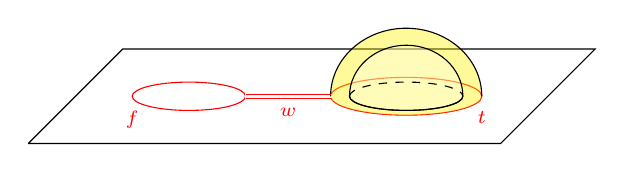
\begin{tikzpicture}[scale=1.2]
      \draw (0, 0) -- (5, 0) -- (6, 1) -- (1, 1) -- (0, 0);

      \draw [red] (4, 0.5) ellipse (0.8 and 0.2);
      \fill [white] (3.19, 0.52) rectangle (3.21, 0.48);

      \begin{scope}[shift={(4, 0.5)}, scale=0.4]
        \fill [yellow, opacity=0.4] (-2, 0) arc (180:0:2 and 1.8) arc(360:180:2 and 0.5);
        \draw (-2, 0) arc (180:0:2 and 1.8);
      \end{scope}
      \begin{scope}[shift={(4, 0.5)}, scale=0.3]
        \draw [fill=white, fill opacity=0.3] (-2, 0) arc (180:0:2 and 1.8) arc(360:180:2 and 0.5);
        \draw (-2, 0) arc (180:360:2 and 0.5);
        \draw [dashed] (-2, 0) arc (180:0:2 and 0.5);
      \end{scope}

      \draw [red] (1.7, 0.5) ellipse (0.6 and 0.15);
      \node [red] at (1.1, 0.25) {\scriptsize $f$};

      \fill [white] (2.29, 0.52) rectangle (2.31, 0.48);
      \draw [red] (2.3, 0.52) -- (3.2, 0.52);
      \draw [red] (2.3, 0.48) -- (3.2, 0.48) node [pos=0.5, below] {\scriptsize $w$};

      \node [red] at (4.8, 0.28) {\scriptsize $t$};
    \end{tikzpicture}
    \caption{A schematic picture of the modification along a $2$-cell in $n = 3$}
  \end{figure}
  For any lift $\tilde{f}$ of $f$, we can pick a lift $\tilde{g}$ that agrees with $\tilde{f}$ on the points $g$ and $f$ agree. This will then have the property that
  \[
    [\tilde{g}] = [\tilde{f}] \pm \gamma' \cdot d_{q + 1}(\phi_j^{q + 1})
  \]
  for some $\gamma' \in \pi_1 W$. Note that we can replace $w$ by composing with any loop, and the result is that $\gamma'$ will be multiplied by the corresponding class. So we can arrange $\gamma'$ to be anything we like. If we precompose $t_j$ by a degree $-1$ diffeomorphism $S^q \to S^q$, then we can change the sign before $\gamma'$ as well.
\end{proof}

Unfortunately, a priori, knowing what value $[f]$ takes in $C_q(\tilde{W}, \widetilde{\partial_0 W})$ is not very useful. This is the problem we discussed before, that in homology, there can be cancellation. To fix this, we use a result known as \emph{Whitney's trick}, which we shall not prove. We shall only state a special case we need:

\begin{thm}[Whitney's trick, {\cite[Theorem 6.6]{milnor-h-cobordism}}]
  Let $n \geq 5$ and $2 \leq q \leq n - 3$. Let $M$ be an $n$-dimensional manifold, $N \subseteq M$ an $(n - q)$-dimensional submanifold, and $f: S^q \to M$ a smooth embedding transverse to $N$.

  Suppose $x, y \in N \cap f(S^q)$ have opposite intersection numbers, and there are paths $\gamma_1, \gamma_2$ from $x$ to $y$ lying in $N$ and $f(S^q)$ respectively such that $\gamma_1 \cdot \gamma_2^{-1}$ is null-homotopic. Then $f$ is isotopic to a map whose intersection with $N$ is exactly $N \cap f(S^q) \setminus \{x, y\}$.\qedhere
\end{thm}

This allows us to prove
\begin{lemma}[Homology lemma]
  Let $n \geq 6$, and suppose
  \[
    W \cong \partial_0 W \times [0, 1] + \sum_{i = 1}^{p_2} (\phi_i^2) + \sum_{i = 1}^{p_3} (\phi_i^3) + \cdots.
  \]
  Fix $2 \leq q \leq n - 3$ and $i_0 \in \{1, 2, \ldots, p_q\}$. Let $f: S^q \to \partial_1 W_q$ be an embedding. Then the following statements are equivalent
  \begin{enumerate}
    \item $f$ is isotopic to an embedding that intersects the transverse sphere of $(\phi_{i_0}^q)$ at one point transversely, and is disjoint from the transverse spheres of the other $q$-handles.
    \item If $\tilde{f}: S^q \to \tilde{W}_q$ is a lift of $f$ to the universal cover, then there is $\gamma \in \pi_1W$ with
      \[
        [\tilde{f}] = \pm \gamma \cdot (\phi_{i_0}^q).
      \]
  \end{enumerate}
\end{lemma}

\begin{proof}
  Recall that if $f$ meets the transverse spheres of $q$-handles transversely at finitely many points $x_{i, j} \in (\phi_i^q)$, then we have
  \[
    [\tilde{f}] = \sum_{x_{i, j}}\varepsilon_{i, j}\cdot \gamma_{i, j}\cdot (\phi_i^q)
  \]
  for some signs $\varepsilon_{i, j} \in \{\pm 1\}$ and $\gamma_{i, j} \in \pi_1 W$. Thus (1) $\Rightarrow$ (2) is clear. For the converse, the fact that $[\tilde{f}]$ is also equal to just $\pm \gamma [\phi_{i_0}^q]$ means there should be a lot of cancellation on the right, which we want to translate to the geometric condition of being able to eliminate the intersections.
  
  To do so, we need to be precise about what these $\gamma_{i, j}$ exactly are. Note that $[\tilde{f}]$ and $(\phi_i^q)$ are only well-defined up to an element $\gamma \in \pi_1 W$. To fix these, we make the following choices. Identifying $S^q$ with its image under $f$, we 
  \begin{itemize}
    \item Pick a basepoint $y \in S^q \subseteq \partial_1 W_q$. 
    \item For each $(\phi_i^q)$, pick a favorite point $z_i$ and a path from $z_i$ to $y$.
    \item For each $x_{i, j}$, pick a path $u_{i, j}$ from $y$ to $x_{i, j}$ in $S^q$.
    \item For each $x_{i, j}$, pick a path $v_{i, j}$ from $x_{i, j}$ to $z_i$ in the transverse sphere of $(\phi_i^q)$.
  \end{itemize}
  The path $\gamma_{i, j}$ is then given by the composition $u_{i, j} \cdot v_{i, j} \cdot w \in \pi_1(W_q, y)$.

  Now by assumption, we have $[\tilde f] = \pm \gamma (\phi_{i_0}^q)$. So we have
  \[
    \pm \gamma \cdot (\phi_{i_0}^q) = \sum_{x_{i, j}} \varepsilon_{i, j} \cdot \gamma_{i, j} \cdot (\phi_i^q).
  \]
  But since $(\phi_i^q)$ form a $\Z[\pi_1 W]$-basis of $C_q(\tilde{W})$, if there is more than one point of intersection, we can find $x_{i, j}$ and $X_{i', j'}$ such that
  \[
    \gamma_{i, j} = \gamma_{i', j'},\quad \varepsilon_{i, j} = - \varepsilon_{i', j'}.
  \]
  Moreover, if we take the explicit representative of $\gamma_{i, j}$ and $\gamma_{i', j'}$ above, we see that $\gamma_{i, j} \cdot \gamma_{i', j'}^{-1}$ is exactly a loop of the sort required by Whitney's trick to eliminate the intersections. So we can inductively remove intersections until we are left with a single point of intersection with $(\phi_{i_0}^q)$.
\end{proof}

With all the tools in place, we can now continue with our original program.
\begin{lemma}[Normal form lemma]\label{lemma:normal-form}
  Let $W$ be an oriented compact $h$-cobordism of dimension $\geq 6$. Fix an integer $q$ with $2 \leq q \leq n - 3$. Then there is a handlebody decomposition with only handles of index $q$ and $q + 1$.
\end{lemma}

\begin{proof}
  Observe that if we have a handlebody decomposition of $W$, then using the symmetry between $n$ and $(n - q)$ in $D^n \times D^{n - q}$, we can ``turn it around'' and view it as a handlebody decomposition of $W$ starting from $\partial_1 W$ instead, and each $q$ handle becomes an $(n - q)$-handle. Morse-theoretically, this is the same as replacing a Morse function $f$ by $-f$. Thus, it suffices to show that we can eliminate all handles of degree $< q$.

  We do this by induction on $q$, where we have already taken care of the $q = 1$ and $q = 2$ case. For higher $q$, we make use of the elimination lemma. Suppose $(\phi^q)$ is a $q$-handle. Then since $H_q(\tilde{W}, \widetilde{\partial_0 W})$ = 0, we know there exists $x_j \in \Z[\pi_1 W]$ such that
  \[
    (\phi^q) = \sum x_j \,\mathrm{d}_{q + 1} (\phi_i^{q + 1}).
  \]
  Take any trivial embedding $\bar{\psi}^{q + 1}$ in $\partial_1^\circ W_q$. Then $[\widetilde{\bar{\psi}^{q + 1}}|_{S^q \times \{0\}}] = 0$. By the modification lemma, there is an embedding $\psi^{q + 1}: S^q \times D^{n - q} \to \partial_1^\circ W_q$ such that
  \[
    [\widetilde{\psi^{q + 1}}|_{S^q \times \{0\}}] = [\widetilde{\bar{\psi}^{q + 1}}|_{S^q \times \{0\}}] + \sum x_j \, \mathrm{d}_{q + 1} (\phi_i^{q + 1}) = (\phi^q).
  \]
  So by the elimination and homology lemmas, we can replace $(\phi^q)$ by a $(q + 2)$-handle.
\end{proof}

\begin{thm}[$s$-cobordism theorem]
  Let $(W, M, N)$ be an $h$-cobordism of dimension $n \geq 6$. Then $W$ is trivial if and only if the Whitehead torsion $\tau(W, M) = 0$.
\end{thm}

\begin{proof}
  Take a handlebody decomposition with handlebodies in degree $q$ and $q + 1$ only, for suitable $q$. Then up to a sign, the Whitehead torsion is the differential in the corresponding CW structure. We know that this differential can be  reduced to nothing via the column operations, multiplication by $\pm g$ for $g \in \pi_1 W$, and reducing
  \[
    \begin{pmatrix}
      A & 0\\
      0 & 1
    \end{pmatrix} \rightsquigarrow A.
  \]
  The ability to perform column operations is given by the modification lemma; multiplication by $\pm g$ is just changing the choice of lifts and has no geometric significance, and the last operation is given by the cancellation lemma. So we can reduce our cobordism to the trivial cobordism.
\end{proof}

Previously when discussing the Whitehead torsion, we promised to prove some existence results about non-trivial Whitehead torsions. With the machinery in place, it is now easy. Given an element $[A] \in \Wh(G)$, pick a manifold with fundamental group $G$ of large dimension, say 57, and then construct a handlebody decomposition with handles of degrees, say, 30 and 31, according to the matrix $A$. This will then be an $h$-cobordism with non-trivial Whitehead torsion.

\section{Siebenmann's end theorem}\label{sec:siebenmann}
We shall use the ideas developed so far to understand the following problem:
\begin{problem}
  Let $M$ be an open manifold possibly with boundary. Can we find a ``completion'' $\bar{M}$, namely a compact manifold with boundary and an inclusion $M \hookrightarrow \bar{M}$ such that $\bar{M} \setminus M$ is a union of boundary components?
\end{problem}
This problem was first solved by Siebenmann in his thesis \cite{siebenmann-thesis}, but the exposition here is based on \cite[Chapter 12]{steve-ferry}.

\begin{eg}
  The surface of infinite genus is not the interior of a manifold with boundary.
\end{eg}

Given an open manifold $M$, we first ask how many \emph{ends} $M$ has:
\begin{defi}
  Let $M$ be an open manifold with boundary. We say $M$ has \emph{$k$ ends} if there is a compact set $K$ such that for any $K' \supseteq K$ compact, the set $M \setminus K'$ has $k$ many unbounded components, i.e.\ components with non-compact closures.
\end{defi}
It is clear that if such a $K$ exists, then $k$ does not depend on the choice of $K$.
\begin{eg}
  $\R \times S^1$ has two ends, while the open disk $\mathring{D}^n$ has one end.
\end{eg}
We would like to focus on the case where there is one end. This is where our assumption that $M$ can have boundary comes in --- we can simply consider (the closure of) each unbounded component of $M \setminus K$ separately. Thus, we from now on assume there is only one end.

To tackle this problem, we first think about what $M$ would look like if it can be completed. The crucial property is that boundaries of manifolds admit collars, i.e.\ if $\partial \bar{M}$ is the (new) boundary of $\bar{M}$, then the inclusion $\partial \bar{M} \hookrightarrow \bar{M}$ extends to an embedding $\partial \bar{M} \times [0, 1] \hookrightarrow \bar{M}$ under the identification $\partial \bar{M} \cong \partial \bar{M} \times \{0\}$. Thus, if $M$ can be completed, we should be able to find a collar $V \subseteq M$ such that $V \cong \partial V \times (0, 1]$, and this is our goal.

This sounds reminiscent of the $s$-cobordism theorem, but there is a key difference, namely that $V$ is not fixed. For example, suppose that we find that $V$ is built by adding three $2$-cells to $(0, 1] \times \partial V$. What we will do is to simply include these $2$-cells in $K$ so that they are no longer part of $V$! Thus, we do not have to assume our end is homologically trivial, but instead we will manually tweak it to get rid of homology.

After we get rid of all homology groups, it turns out we need not worry about problems of Whitehead torsion, since we can always push them away to infinity. This is made precise by the following lemma:
\begin{lemma}\label{lemma:end-simplify}
  Suppose we have an infinite sequence
  \[
    V = V_1 \supseteq V_2 \supseteq \cdots
  \]
  of connected submanifolds such that
  \begin{enumerate}
    \item $\bigcap V_i = 0$
    \item $\pi_1(V_{i + 1}) \to \pi_1(V_{i})$ is an isomorphism for all $i$
    \item The inclusions $\partial V_i \to V_i$ are homotopy equivalences for all $i$.
  \end{enumerate}
  Then $V \cong \partial V \times [0, 1)$.
\end{lemma}

\begin{proof}
  Take $C_i = V_i \setminus \mathring{V_{i + 1}}$. Then by the homology long exact sequence for $(\tilde{V}_i, \tilde{C}_i, \widetilde{\partial V_i})$ and excision $H_k(\tilde{V}_i, \tilde{C}_i) \cong H_k(\tilde{V}_{i + 1}, \widetilde{\partial V_{i + 1}})$, we know that $H_*(\tilde{C}_i, \widetilde{\partial V}_i) = 0$ for all $i$. So each $\tilde{C}_i$ is an $h$-cobordism. Picking a collar neighbourhood of $\partial V_2$, we can schematically describe our $V$ as
  \begin{center}
    \begin{tikzpicture}[yscale=0.7]
      \draw (6.5, 0) -- (0, 0) -- (0, 2) -- (6.5, 2);
      \draw (6, 0) -- (6, 2);

      \draw (2, 0) -- (2, 2);
      \node at (1, 1) {$C_1$};
      \draw (4, 0) -- (4, 2);
      \node at (3, 1) {triv};

      \node at (5, 1) {$C_2$};
      \node at (8, 1) {$\cdots$};
      \draw [path fading=east] (6.5, 2) -- (7.5, 2);
      \draw [path fading=east] (6.5, 0) -- (7.5, 0);
    \end{tikzpicture}
  \end{center}
  The point is that the Whitehead torsion is additive, so we can find a $-C_1$ with $\tau(-C_1) = - \tau(C_1)$, so that $C_1 \cup -C_1$ and $-C_1 \cup C_1$ are trivial. We can then describe our above cobordism as
  \begin{center}
    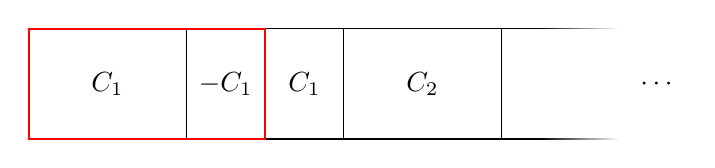
\begin{tikzpicture}[yscale=0.7]
      \draw (6.5, 0) -- (0, 0) -- (0, 2) -- (6.5, 2);
      \draw (6, 0) -- (6, 2);

      \draw (2, 0) -- (2, 2);
      \node at (1, 1) {$C_1$};
      \draw (3, 0) -- (3, 2);
      \draw (4, 0) -- (4, 2);
      \node at (2.5, 1) {$-C_1$};
      \node at (3.5, 1) {$C_1$};

      \node at (5, 1) {$C_2$};
      \draw [red, thick] (0, 0) rectangle (3, 2);
      \node at (8, 1) {$\cdots$};
      \draw [path fading=east] (6.5, 2) -- (7.5, 2);
      \draw [path fading=east] (6.5, 0) -- (7.5, 0);

    \end{tikzpicture}
  \end{center}
  We can now define a diffeomorphism $\partial V \times [0, \frac{1}{2}] \to \overline{C_1 \cup -C_1}$. We then rename $C_1 + C_2$ as $C_2$, construct a diffeomorphism $\partial V \times [\frac{1}{2}, \frac{3}{4}] \to \overline{C_2 \cup -C_2}$, and keep going on until we get a diffeomorphism $\partial V \times [0, 1) \to V$.
\end{proof}

\begin{defi}
  Let $M$ be as before. A neighbourhood of infinity is a closed connected submanifold $V \subseteq M$ (with boundary) such that $\overline{M \setminus V}$ is compact.
\end{defi}

There will always be situations such as the surface of infinite genus where there is no hope in finding a collar. Thus, we need to impose the following condition.
\begin{defi}
  We say (the end of) $M$ is \emph{strongly tame} if every neighbourhood of infinity has the homotopy type of a finite CW complex.
\end{defi}
This is not a standard definition. Instead, in the literature, it is more common to require that the neighbourhoods are finitely dominated, and then there will be an obstruction to finding a collar, namely Wall's finiteness obstruction. In our case, since we assumed the neighbourhoods are in fact finite CW complexes, there is no obstruction.

Observe that we don't have to manually check \emph{all} neighbourhoods of infinity. If $V \supseteq V'$ are neighbourhoods of infinity, then $V$ is obtained from $V'$ by attaching finitely many cells, since the difference is a compact manifold. So if $V'$ is finite, then so is $V$. Thus, we only have to show that there are arbitrarily small neighbourhoods of infinity that are finite.

%\begin{lemma}
%  Let $V$ be a neighbourhood of infinity. Then the following are equivalent:
%  \begin{enumerate}
%    \item There is a homotopy $H: [0, 1] \times V \to V$ such that $H(0, x) = x$ and $H(1, -)$ has precompact image.
%    \item $V$ is finitely dominated.
%  \end{enumerate}
%\end{lemma}
%
%\begin{defi}
%  We say (the end of) $M$ is \emph{tame} if the conditions of the lemma hold for all neighbourhoods of infinity.
%\end{defi}
%Observe that if $V \supseteq V'$ are neighbourhoods of infinity, and $V'$ satisfies (1), then the homotopy extension property of $\partial V' \hookrightarrow \overline{V \setminus V'}$ implies $V$ also satisfies (1), and so we only have to check that there are arbitrarily small neighbourhoods of infinity for which (1) holds.
%
%\begin{proof}\leavevmode
%  \begin{itemize}[leftmargin=2.2cm]
%    \item[(1) $\Rightarrow$ (2)] Let $D$ be a compact submanifold of $V$ containing the image of $H(1, -)$. Then $D$ is a finite CW complex and then the composition
%      \[
%        V \overset{\tilde{H}(1, -)}{\longrightarrow} D \longhookrightarrow V
%      \]
%      is homotopic to the identity via $H$.
%    \item[(2) $\Rightarrow$ (1)] If we have a finite domination
%      \[
%        V \overset{s}{\longrightarrow} D \overset{r}{\longrightarrow} V,
%      \]
%      then by definition there is a homotopy $H$ as required with $H(1, -) = r \circ s$, and thus the image is contained in the compact set $r(D)$.\qedhere
%  \end{itemize}
%\end{proof}

As before, it is very important to consider the fundamental group. Intuitively, we want to talk about the ``fundamental group at infinity'', but this is not a group in general. Instead, it is a pro-group.
\begin{defi}
  A pro-group is an infinite sequence of groups
  \[
    G_1 \leftarrow G_2 \leftarrow G_3 \leftarrow \cdots.
  \]
  Equivalence of pro-groups is the equivalence relation generated by the following two relations:
  \begin{itemize}
    \item Isomorphisms as diagrams of groups
    \item Passing on to subsequences (and composing the relevant maps).
  \end{itemize}
  A pro-group is \emph{stable} if it is equivalent to a constant sequence
  \[
    G \leftarrow G \leftarrow G \leftarrow \cdots.
  \]
  Since equivalent pro-groups have the same inverse limit, we can recover $G$ by
  \[
    G = \varprojlim G_i.
  \]
\end{defi}
Note that it is important that we talk about the equivalence relation generated by these two operations. It is possible that two equivalent pro-groups have no groups in common, since we can pass on to a super-sequence and then remove the things that were originally there. For example, for any group $G$, the pro-group
\[
  G \overset{0}{\leftarrow} G \overset{0}{\leftarrow} G \overset{0}{\leftarrow} G \overset{0}{\leftarrow} \cdots
\]
is pro-equivalent to constant zero sequence.

The following is easy to verify:
\begin{fact}
  Pro-groups $\{G_i\}$, $\{H_i\}$ are equivalent iff there exists subsequences $\{G_{i_k}\}$, $\{H_{j_k}\}$ and a commutative diagram
  \[
    \begin{tikzcd}[column sep=tiny]
      G_{i_1} && G_{i_2} \ar[ll] \ar[ld] && G_{i_3} \ar[ll] \ar[ld] && G_{i_4} \ar[ll] \ar[ld] && \cdots \ar[ll]\\
      & H_{j_1} \ar[lu] && H_{j_2} \ar[ll] \ar[lu] && H_{j_3} \ar[ll] \ar[lu] && H_{j_4} \ar[ll] \ar[lu] && \cdots \ar[ll]
    \end{tikzcd}
  \]
\end{fact}

\begin{defi}
  Let $M$ be as before, and $\{V_i\}$ a nested collection of neighbourhoods at infinity with $\bigcap V_i = \emptyset$. For each $V_i$, pick a base point $x_i$, and pick paths $\gamma_i$ from $x_i$ to $x_{i + 1}$. The pro-group associated to $\{(V_i, x_i, \gamma_i)\}$ is
  \[
    \pi_1(V_1, x_1) \overset{f_1}\longleftarrow \pi_1(V_2, x_2) \overset{f_2}\longleftarrow \pi_1(V_3, x_2) \overset{f_3}\longleftarrow \cdots.
  \]
\end{defi}

In general, this pro-group depends on the choice of the paths $\gamma_i$. If we pick different paths, then we replace each $f_i$ by some conjugate. Fortunately, we have the following easy, purely algebraic result:
\begin{fact}\label{fact:pro}
  If $\{(G_i, f_i)\}$ is a stable pro-group, and $g_i \in G_i$, then $\{(G_i, g_i f_i g_i^{-1})\}$ is also a stable pro-group with the same inverse limit.\fakeqed
\end{fact}

Finally, observe that if $\{V_i\}, \{W_i\}$ are nested neighbourhoods of infinity with $\bigcap V_i = \bigcap W_i = \emptyset$, then after passing on to subsequences, we may assume
\[
  V_1 \supseteq W_1 \supseteq V_2 \supseteq W_2 \supseteq \cdots,
\]
and so the induced pro-groups are equivalent by \Cref{fact:pro}. Thus, it is sensible to define
\begin{defi}
  Let $M$ be as before. We say $M$ has stable fundamental group at infinity if the pro-group associated to any (hence all) $\{(V_i, x_i, \gamma_i)\}$ is stable, and the inverse limit $\pi_1 \varepsilon$ is called the fundametnal group at infinity.
\end{defi}

Again, it is clear that if $M$ has a collar, then it has stable fundamental group at infinity. One might think that tameness guarantees this is the case, but unfortunately for us, this is not the case, and we must impose this as an extra condition (see \cite[Example 3]{manifold-non-stable}).

From now on, we assume $M$ has dimension $n \geq 6$ and is one-ended, strongly tame and with stable fundamental group at infinity. We shall proceed to find a collar.
\begin{defi}
  A $1$-neighbourhood of infinity is a $V \subseteq M$ such that $\pi_1 \partial V \cong \pi_1 V \cong \pi_1 \varepsilon$ under the obvious maps.
\end{defi}

\begin{prop}
  There are arbitrarily small $1$-neighbourhoods of infinity.
\end{prop}
This relies on the following (less easy) algebraic lemma, which we still won't prove:
\begin{lemma}
  Let $G, H$ be finitely presented groups and $f: G \to H$ a surjective homomorphism. Then $\ker f$ is normally generated by finitely many elements.\fakeqed
\end{lemma}
This is equivalent to the perhaps more familiar fact that a finitely presentable group is finitely presented under any choice of (finitely many) generators, by precomposing with a surjection from a finitely generated free group to $G$.

\begin{proof}[Proof of proposition]
  By assumption of stability of $\pi_1$, we can find arbitrarily small neighbourhoods $U \supseteq V$ such that we have a commutative diagram
  \[
    \begin{tikzcd}[column sep=tiny]
      & \pi_1 U \ar[ld] & & \pi_1 V \ar[ld] \ar[ll]\\
      \pi_1 \varepsilon & & \pi_1 \varepsilon \ar[ll, "1"'] \ar[ul] & & \pi_1 \varepsilon \ar[ll, "1"'] \ar[ul]
    \end{tikzcd}
  \]
  We wish to first make $\pi_1 V \to \pi_1 \varepsilon$ an isomorphism. We know this is surjective, and the kernel is normally generated by finitely many loops $\{\gamma_i\}$. Moreover, since these also lie in the kernel of the map $\pi_1 V \to \pi_1 U$, they bound disks in $U$. Since $n$ is large enough, we may assume these disks are embedded and disjoint. Then add tubular neighbourhoods of these disks to $V$. Again since $n$ is large enough, this doesn't affected the connectedness of $\partial V$, and Seifert-van Kampen implies we now have $\pi_1 V \to \pi_1 \varepsilon$ an isomorphism.

  We next want to ensure $\pi_1 \partial V \to \pi_1 V$ is an isomorphism. We first arrange it to be a surjection. Fix a basepoint in $\partial V$. If we have any loop $[\gamma] \in \pi_1 V$, we can pick an embedding in $V$ and remove a tubular neighbourhood of it. Then $\partial V$ will now have a loop homotopic to $\gamma$, and again Seifert--van Kampen implies the fundamental group of $\pi_1V$ is unchanged. Since $\pi_1 V$ is finitely generated, we only need to do this finitely many times and the map will be surjective.

  Finally, we need to clear the kernel of $\pi_1 \partial V \to \pi_1 V$. This is again finitely generated by the above lemma. So for each generator $[\gamma]$ of the kernel, embed a disk in $V$ that kills of $\gamma$, and remove a tubular neighbourhood.
\end{proof}
We want to perform a similar procedure to get rid of higher relative homology groups. As in the case of Wall's finiteness obstruction, we really don't have to take much care until we hit the top dimension. We may na\"ively think the top dimension is $n$, but in fact, it is $n - 2$. The reason is that if we think of the end as a cobordism, then adding $n - 1$ or $n$ cells would change the $\pi_1$ and $\pi_0$ of the ending manifold.

\begin{lemma}
  Let $V$ be a $1$-neighbourhood of $M$. Then $(V, \partial V)$ has the homotopy type of a finite CW complex of dimension $n - 2$.
\end{lemma}

\begin{proof}
  By \Cref{cor:dim-dom-rel}, we only have to show that $(V, \partial V)$ is dominated rel $\partial V$ by a finite relative CW complex.

  Let $V'$ be another $1$-neighbourhood contained in $V$. Let $C = V \setminus \mathring{V}'$. Then $(C, \partial V, \partial V')$ is a cobordism, and Seifert--van Kampen applied to $V = C \cup_{\partial V'} V'$ tells us
  \[
    \pi_1 C \cong \pi_1(\partial V').
  \]
  So if we think of $C$ as a cobordism starting from $\partial V'$, then $\partial V' \hookrightarrow C$ is $1$-connected, and we can find a handlebody decomposition with no $0$- or $1$-handles. Thus, in the dual handlebody decomposition, $C$ is built from $V$ by adding handles up to dimension $n - 2$. So $(C, \partial V)$ is a handlebody decomposition with cells of dimension $\leq n - 2$. In particular, it is a finite relative CW complex of dimension $\leq n - 2$. We will show that for an appropriate $V'$, this dominates $V$.

  We are actually almost done, but since we want our homotopies to fix $\partial V$, we need to do things in a slightly funny way. Fix a proper sub-$1$-neighbourhood $V'$ of $V$. By assumption, there is a homotopy equivalence
  \[
    \begin{tikzcd}
      X \ar[r, yshift=2, "f"] & V' \ar[l, yshift=-2, "g"]
    \end{tikzcd}
  \]
  with $X$ a finite CW complex. The image of $f$ is compact, and so we can find an even smaller $1$-neighbourhood $V''$ such that $\im(f) \subseteq V' \setminus V''$. Then $V' \setminus V''$ dominates $V'$ via
  \[
    \begin{tikzcd}
      V' \ar[r, "f \circ g"] & V' \setminus V'' \ar[r, hook] & V'.
    \end{tikzcd}
  \]
  By the homotopy extension property, we know that $V \setminus V''$ dominates $V$ rel $\partial V$, and $V \setminus V''$ has the homotopy type of a finite relative CW complex with cells of dimension $\leq n - 2$.
\end{proof}

With this understanding, we are now ready to prove Siebenmann's end theorem.
\begin{thm}[\cite{siebenmann-thesis}]\label{thm:end}
  Let $M$ be one-ended, $n = \dim M \geq 6$, strongly tame, and with stable fundamental group at infinity. Then $M$ has a collar.
\end{thm}

The idea of the proof is to just kill off relative homology groups as above, but we have trouble turning the disks representing relative homology classes into smooth embeddings in high dimension. The trick is to take handlebody decompositions of $V$, which give us relatively concrete handles that we can excise away from $V$.

%We can perform similar manipulations kill off relative homology groups one by one, using the Hurewicz isomorphism
%\[
%  \pi_k(V, \partial V) \cong \pi_k(\tilde{V}, \widetilde{\partial V}) \to H_k(\tilde{V}, \widetilde{\partial V}).
%\]
%To be precise, for each generator of $H_k(\tilde{V}, \widetilde{\partial V})$, pick a map $(D^k, \partial D^k) \to (V, \partial V)$ representing it, make it into an embedding, and then excise tubular neighbourhoods. Finite domination ensures we only have finitely many things to kill. However, we have the problem that standard embedding theorems no longer let us turn our disks into embeddings when $k > \frac{n}{2}$.

\begin{proof}
  By \Cref{lemma:end-simplify}, it suffices to find arbitrarily small $1$-neighbourhoods $V$ such that $\partial V \hookrightarrow V$ is a homotopy equivalence, or equivalently, such that their universal covers have trivial relative homology.

  Start with $V$ a $1$-neighbourhood. We will inductively show that we can modify $V$ such that $H_\ell(\tilde{V}, \widetilde{\partial V}) = 0$ for $\ell \leq k$. Assume this holds for all $\ell < k$, and we want to make it true for $\ell = k$. We will assume $k < n - 2$, since for $k = n - 2$, a bit more care is needed at some places.

  Since singular chains are compact, and $H_k(\tilde{V}, \widetilde{\partial V})$ is finitely generated, we can find some other neighbourhood $V' \subseteq V$ such that if $C = V \setminus \mathring{V'}$, then
  \[
    H_k(\tilde{C}, \widetilde{\partial V}) \to H_k(\tilde{V}, \widetilde{\partial V})
  \]
  is surjective. Moreover, by induction, we may assume $H_\ell(\tilde{V'}, \widetilde{\partial V'}) = 0$ for $\ell < k$.

  Sadly, the long exact sequence for $(\tilde{V}, \tilde{C}, \widetilde{\partial V})$ only tells us
  \[
    H_\ell(\tilde{C}, \widetilde{\partial V}) = 0\text{ for }\ell < k - 1.
  \]
  Thus, we can take a handlebody decomposition of $(C, \partial V)$ with only cells of dimension $\geq k - 1$, and we need to be careful about the $(k - 1)$-handles.

  Suppose we have a homology class $[c] \in H_k(\tilde{C}, \widetilde{\partial V})$ that is represented by a single handle $\phi$. Then since $\d_k (\phi) = 0$, Whitney's trick lets us modify $\phi$ so that the attaching map does not intersect the transverse spheres of the $(k-1)$-handles, and then by applying a flow, we may assume it doesn't hit any of the $(k - 1)$-handles at all. Removing $\phi$ from $V$ then kills off the homotopy class $[c]$ in $H_k(\tilde{C}, \widetilde{\partial V})$.

  In general, if we have
  \[
    [c] = \sum n_i \gamma_i (\phi_i),\quad n_i \in \Z,\quad \gamma_i \in \pi_1 \varepsilon,
  \]
  what we do is that we introduce a cancelling pair of $k$- and $(k + 1)$-handles, say $\phi$ and $\psi$. We can then modify the attaching map of $\phi$ as in the proof of the \hyperref[lemma:modification]{Modification Lemma} to add $g_i \phi_i$ with the appropriate multiplicities. Then $\phi$ would represent the class $[c]$ (the job of $\psi$ is now to identify $(\phi)$ with $\sum n_i \gamma_i (\phi_i)$). We then excise $\phi$ as above.

  Since $H_k(\tilde{C}, \widetilde{\partial V})$ is finitely generated, we only have to excise a finite number of such handles, and the induction step is completed.

  At $k = n - 2$, we need to take a bit of care. To ensure we do not introduce extra homology in higher dimensions, we must ensure $H_k(\tilde{V}, \widetilde{\partial V})$ is a free $\Z[\pi_1 \varepsilon]$-module. Recall that $(V, \tilde{\partial V})$ has the homotopy type of a relative CW complex of dimension $\leq n - 2$, with trivial homology in degrees $< n - 2$. So as in the case of Wall's finiteness obstruction, we deduce that $H_k(\tilde{V}, \widetilde{\partial V})$ is stably free. We can then excise trivial $(n - 3)$-handles to make this actually free.

  To eliminate $H_{n - 2}(\tilde{V}, \widetilde{\partial V})$, we can no longer apply the procedure above, since we do not want to introduce $(n - 1)$-handles, which could potentially mess up our $\pi_1$. So we have to be a bit more careful (excising $(n - 2)$-handles is itself an operation that could potentially mess up $\pi_1$. But we have hope if we don't mess up so much). As above, pick a smaller neighbourhood $V'$ such that $H_{n - 2}(\tilde{C}, \widetilde{\partial V}) \to H_{n - 2}(\tilde{V}, \widetilde{\partial V})$ is surjective. Then the long exact sequence
  \[
    0 \to H_{n - 2}(\tilde{C}, \widetilde{\partial V}) \to H_{n - 2}(\tilde{V}, \widetilde{\partial V}) \to H_{n - 2}(\tilde{V}, \tilde{C}) \to H_{n - 3}(\tilde{C}, \widetilde{\partial V}) \to 0
  \]
  shows that the first, and hence the last map are both isomorphisms. Hence (by excising trivial handles from $V'$) we may assume that $H_k(\tilde{C}, \widetilde{\partial V})$ is free for $k = n - 2$ and $n - 3$, and vanishes otherwise.

  As in the normal form lemma \ref{lemma:normal-form}, we may pick a handlebody decomposition of $(C, \partial V)$ with handles concentrated in degree $n - 3$ and $n - 2$. Then the exact sequence
  \[
    0 \to H_{n - 2}(\tilde{C}, \widetilde{\partial V}) \to C^{\cell}_{n - 2}(\tilde{C}, \widetilde{\partial V}) \to C^{\cell}_{n - 3}(\tilde{C}, \widetilde{\partial V}) \to H_{n-3}(\tilde{C}, \widetilde{\partial V}) \to 0
  \]
  splits by freeness. In particular, $H_{n - 2}(\tilde{C}, \widetilde{\partial V})$ is a direct summand of $C^{\cell}_{n-2}(\tilde{C}, \widetilde{\partial V})$. We want to arrange the handles so that a subset of them forms a basis of $H_{n - 2}(\tilde{C}, \widetilde{\partial V})$.
  
  This is purely algebraic. Pick any basis $a$ of $H_{n - 2}(\tilde{C}, \widetilde{\partial V})$, and complete this to a basis $a \cup b$ of $C^{\cell}_{n - 2}(\tilde{C}, \widetilde{\partial V})$. Then under $a \cup b$, the basis of $C^{\cell}_{n - 2}(\tilde{C}, \widetilde{\partial V})$ under the handlebody decomposition is given by an invertible matrix, say $M$. We now add $|a \cup b|$ many cancelling $(n - 2)$- and $(n - 3)$- pairs, so that the matrix is now of the form
  \[
    \begin{pmatrix}
      M & 0\\
      0 & I
    \end{pmatrix}.
  \]
  We would be done if we can perform elementary row and column operations (via the modification lemma) so that the top left-hand corner is an $I$ instead, the bottom right-hand corner can be anything, and top-right corner vanish. This is possible by elementary linear algebra (this requires $M$ to be invertible, which is why we didn't do this in the past).

  Once this is done, we can then apply Whitney trick and excise these handles as above. To conclude the theorem, we need to check that the result $U$ is still a $1$-neighbourhood. To see this, observe that it is clear that $\partial U \to U$ preserves $\pi_1$, since $U$ is obtained from $\partial U$ by adding $(n - 3)$- and $(n - 2)$-handles. Similarly, $\pi_1(\partial U) \cong \pi_1(C \cap U)$. On the other hand, $C \cap U$ is obtained from $\partial V'$ by adding $2$- and $3$-handles, so $\pi_1(\partial V') \to \pi_1(C\cap U)$ is surjective. But the composition
  \[
    \pi_1(\partial V') \to \pi_1(C \cap U) \to \pi_1C \to \pi_1 V
  \]
  is an isomorphism. So $\pi_1(\partial V') \to \pi_1(C \cap U)$ is also injective. Then we are done.

%  The desired result then follows from the next purely algebraic lemma (plus the modification lemma and introduction of trivial $(n - 3)$- and $(n - 2)$- pairs):
%   Under this CW decomposition, the sequence
%  \[
%    0 \to H_{n - 2}(\tilde{C}, \widetilde{\partial V}) \to C^{\cell}_{n - 2}(\tilde{C}, \widetilde{\partial V}) \to C^{\cell}_{n - 3}(\tilde{C}, \widetilde{\partial V}) \to H_{n-3}(\tilde{C}, \widetilde{\partial V}) \to 0
%  \]
%  splits by freeness.
%
%  We now take a basis of $H_k(\tilde{V}, \widetilde{\partial V})$ and perform the same steps as above to find a collection of handles that represent this basis. Note that the attaching map of an $(n - 2)$-handle is a map from $S^{n - 3} \times D^2$, and so we can apply Whitney's trick.
  
%  Keep in mind performing these steps do \emph{not} change the diffeomorphism type of $(C, \partial V)$. We are just finding different ways of looking at $(C, \partial V)$, and ultimately found one where our favorite basis is represented by concrete handles. In this picture, $C$ is obtained from $\partial V$ by first attaching some $(n - 2)$-handles representing the basis, and then some more $(n - 3)$- and $(n - 2)$-handles (we can assume there is no $(n - 1)$ handle as we can replace them by $(n - 3)$-handles, by considering the dual handlebody decomposition and the fact that $\partial V' \hookrightarrow C$ induces isomorphism on $\pi_1$).
%  Keep in mind performing these steps do \emph{not} change the diffeomorphism type of $(C, \partial V)$. We are just finding different ways of looking at $(C, \partial V)$, and ultimately found one where our favorite basis is represented by concrete handles. In this picture, $C$ is obtained from $\partial V$ by first attaching some $(n - 2)$-handles representing the basis, and then some more $(n - 3)$-, $(n - 2)$- and $(n - 1)$-handles.

%  \todo[inline]{Fix this}
%  We now remove these $(n - 2)$-handles, and let $U$ be the result. It is automatic from Seifert--van Kampen that $\pi_1V \cong \pi_1 U$, but it is not automatic that $\pi_1 (\partial V) \cong \pi_1 (\partial U)$, and this is something we must additionally check. This, fortunately, is easy, since $U$ is obtained from $\partial U$ by adding many handles of index $\geq n - 3$, and so $\pi_1 (\partial U) \cong \pi_1 U$.
%
%  To check that this is indeed the case, observe that $C \cap U$ is a cobordism between $\partial U$ and $\partial V'$, and we want to show that the maps in
%  \[
%    \pi_1(\partial U) \to \pi_1 (C \cap U) \to \pi_1(C) \cong \pi_1(\partial V') 
%  \]
%  are isomorphisms. These follow from the following observations:
%  \begin{itemize}
%    \item $C \cap U$ is obtained from $\partial U$ by attaching handles of large dimension. So $\pi_1(\partial U) \cong \pi_1(C\cap U)$.
%    \item In the dual handlebody decomposition, $C \cap U$ is obtained from $\partial V'$ by adding $2$- and $3$-handles. So $\pi_1(\partial V') \to \pi_1(C \cap U)$ is surjective. But the composition
%  \end{itemize}
\end{proof}

It is interesting to ask ourselves, how many ways are there to complete $M$ to a manifold with boundary? The first guess might be that it is unique, but it turns out not. Suppose we complete $M$ into $\bar{M} = M \cup E$. Given any $h$-cobordism $N$ with $\partial_0 N = E$, we can form
\[
  \bar{M}' = \bar{M} \cup_E N.
\]
This is in fact another completion of $M$. Indeed, using the trick in \Cref{lemma:end-simplify}, we see that $N \setminus \partial_1 N \cong \partial_0 N \times [0, 1)$, and so
\[
  \bar{M'} \setminus \partial_1 N \cong \bar{M} \cup E \times [1, 0) \cong M.
\]
The problem of classifying all completions is a bit more subtle, since one has to be very precise about what it means for two completions to be the same. The reader is referred to Siebenmann's original thesis \cite{siebenmann-thesis} for more details.

\section{Fibering over a circle}
Let $M$ be a (connected) manifold, and $\theta \in H^1(M, \Z)$ a cohomology class. Since $S^1$ is a $K(\Z, 1)$, we know $\theta$ is represented by a homotopy class of maps $f: M \to S^1$. The question we want to answer is
\begin{problem}
  When is a map $f: M \to S^1$ homotopy equivalent to a fiber product projection?
\end{problem}

There is a more geometric way to look at this. The Pontryagin--Thom construction tells us the datum of $f$ is equivalent to a framed cobordism class of codimension $1$ submanifolds of $M$. If $f$ were a fiber product, then the corresponding submanifold is the fiber $F$ of any point in $S^1$. Let $M_F$ be the closed manifold with boundary resulting from cutting $M$ along $F$. Then $M_F$ is a fiber bundle over $[0, 1]$, which must be trivial. Hence $M_F \cong F \times [0, 1]$. Conversely, given a framed codimension $1$ submanifold $F$ of $M$, if $M_F \cong F \times [0, 1]$, then $M$ is naturally fibered over $S^1$ using the projection map $F \times [0, 1] \to [0, 1]$.

Thus, we can equivalently view this problem as: given a framed codimension $1$ submanifold of $M$, can we do framed surgery on $F$ so that $M_F$ becomes a product? Given the $s$-cobordism theorem, this is equivalent to asking $F \hookrightarrow M_F$ to be a homotopy equivalence, and some obstruction vanishing.

Recall that in the end theorem, if $\partial V \hookrightarrow V$ fails to be a homotopy equivalence, our strategy was to find some disks representing a non-trivial homology classes, and then throw it out of $V$. In this case, if $F \hookrightarrow M_F$ fails to be a homotopy equivalence, the idea is to take out a cell on one end and put it back on the other, in hope of making $M_F$ looking more like a product.

Unsurprisingly, this does not always work. Observe that if $f$ were homotopic to a fiber bundle projection, then we know what the homotopy type of the fiber would be. We can construct the pullback
\[
  \begin{tikzcd}
    X \ar[r] \ar[d] & M \ar[d, "f"]\\
    \R \ar[r] & S^1
  \end{tikzcd}
\]
where the bottom map is the universal covering map. Since $\R$ is contractible, we know $X$ is the homotopy fiber of $f: M \to S^1$, and hence has the homotopy type of the actual fiber if $f$ were a fiber bundle projection. Equivalently, the pullback depends only on the homotopy class of $f$, and if $f$ were a fiber bundle projection, then $X = F \times \R \simeq F$.

In any case, we have a homotopy long exact sequence
\[
  0 = \pi_2S^1 \to \pi_1X \to \pi_1M \to \pi_1S^1 \to \pi_0X \to \pi_0M = *
\]
From this, we see that $X$ is connected iff $f_*: \pi_1(M) \to \pi_1(S^1)$ is surjective. If it were the zero map, then $X$ would have infinitely many components, and we would be very sad and give up. If not, the image is $n \Z$ for some $n \in \Z$. Then $f$ lifts along the $n$-fold covering map $n: S^1 \to S^1$, and then the map to this cover would be surjective on $\pi_1$. Since $n: S^1 \to S^1$ itself is a fiber bundle projection, there is no lost in generality if we only consider cases where $X$ is connected, i.e.\ $f_*$ is surjective. In this case,
\[
  \pi_1X = \ker (f_*: \pi_1 M \to \pi_1 S^1).
\]
Observe that $X$ is in fact completely determined by $\pi_1X$ as a subgroup of $\pi_1 M$, since it is the covering space corresponding to that subgroup.

If we want $X$ to have the homotopy type of the fiber, which has to be a compact manifold, then we must require that $X$ has the homotopy type of a finite CW complex. The following (non-manifold) example illustrates an example where this fails (the vertical map on the right collapses the left-hand side to a point, and acts as the identity on the right)
\begin{center}
  \begin{tikzpicture}[scale=0.7]
    \draw [semithick] (0, 0) .. controls (1, 1) and (2, 1) .. (2, 0) .. controls (2, -1) and (1, -1) .. (0, 0);
    \draw [semithick, xscale=-1] (0, 0) .. controls (1, 1) and (2, 1) .. (2, 0) .. controls (2, -1) and (1, -1) .. (0, 0);
    \node [circ] at (0, 0) {};

    \draw [commutative diagrams/.cd, every arrow] (0, -1.2) -- (0, -2.8);
    \begin{scope}[shift={(0, -4)}]
      \node [circ] at (0, 0) {};
      \draw [semithick] (0, 0) .. controls (1, 1) and (2, 1) .. (2, 0) .. controls (2, -1) and (1, -1) .. (0, 0);
    \end{scope}

    \begin{scope}[shift={(-10, -4)}]
      \draw [semithick] (-3, 0) -- (3, 0);
      \foreach \x in {-2, 0, 2} {
        \node [circ] at (\x, 0) {};
      }
    \end{scope}

    \begin{scope}[shift={(-10, 0)}]
      \draw [semithick] (-3, 0) -- (3, 0);
      \foreach \x in {-2, 0, 2} {
        \node [circ] at (\x, 0) {};
        \draw [shift={(\x, 0)}, rotate=90, semithick] (0, 0) .. controls (1, 1) and (2, 1) .. (2, 0) .. controls (2, -1) and (1, -1) .. (0, 0);
      }
    \end{scope}
    \draw [commutative diagrams/.cd, every arrow] (-10, -1.2) -- (-10, -2.8);

    \draw [commutative diagrams/.cd, every arrow] (-5.5, 0) -- (-3.5, 0);
    \draw [commutative diagrams/.cd, every arrow] (-5.5, -4) -- (-3.5, -4);
  \end{tikzpicture}
\end{center}
Thus, from now on, we assume $X$ has the homotopy type of a finite CW complex.

In general, it is a better idea to work directly on $X$ itself. To see this, pick a smooth approximation of $f$; pick a regular value $p$; and set $F = f^{-1}(\{p\})$. Let $\tilde{F}$ be a lift of $F$ to $X$. Then $\tilde{F}$ cuts $X$ into two parts, say $X_+$ and $X_-$. Then as before, we can move handles from $X_+$ to $X_-$ and vice versa, and it is very easy to understand what this does to the homology of $X_+$ and $X_-$. If we worked with $M_F$ directly, then the change in homology is less well-understood, since we add the cells back on the other side.

At this point, there are two possible directions we can take:
\begin{enumerate}
  \item We can proceed just as before, using the finiteness hypothesis to move handles across $F$ and hope that we can get rid of all homology.
  \item We apply Siebenmann's end theorem to show that $X$ is abstractly isomorphic to $F \times \R$ for some $F$. This comes with a natural projection map to $\R$, but in general is not the same as original projection $X \to \R$. We then try to relate these two maps, and if we are successful, this would imply $f: M \to S^1$ is homotopic to a fiber bundle projection.
\end{enumerate}
In each case, we are going to encounter some obstruction, depending on $\pi_1 X$. After encountering such obstruction, one has to show that it is a genuine obstruction, i.e.\ it is a well-defined function of the map $f$. If we can do so, we consider the problem solved.

These obstructions are slightly more subtle than the usual ones, since $X$ comes with the action of $\Z = \pi_1S^1$ via deck transformations over $M$, which gives our obstructions extra structures and properties. To avoid dealing with extra complications, we will focus on the case where $\pi_1 X = 0$, in which case the obstruction groups all vanish. We will also assume $M$ has no boundary, which is more for notational convenience than technical convenience. We also assume $\dim M \geq 6$.

For more sophisticated versions, see \cite{browder-levine}, \cite{farrell-fiber}, \cite{siebenmann-fiber}. The approach in \cite{browder-levine} is very similar to ours, but they work with manifolds with boundary as well. In \cite{farrell-fiber}, they attack the problem honestly for general $\pi_1$ along the lines of (1). In \cite{siebenmann-fiber}, the same problem is approached along the lines of (2).

The steps we perform are similar to the proof the Siebenmann's theorem, but they have to be modified appropriately to take care of the deck transformations. Let $T$ be the deck transformation corresponding to a generator of $\pi_1S^2$. Recall that we defined $M_F$ to be the result of splicing $M$ apart at $F$. Fix a lift of $M_F$ to $X$, and label the two ends of $M_F$ as $F_0$ and $F_1$, so that $TF_0 = F_1$. For $r \in \Z$, we define
\[
  M_F^r = \bigcup_{k < r} T^k M_F.
\]
\begin{center}
  \begin{tikzpicture}[xscale=1.5]
    \draw (-3.5, -1) -- (3.5, -1);
    \draw (-3.5, 1) -- (3.5, 1);
    \draw [path fading=east] (3.5, 1) -- (4, 1);
    \draw [path fading=east] (3.5, -1) -- (4, -1);
    \draw [path fading=west] (-3.5, 1) -- (-4, 1);
    \draw [path fading=west] (-3.5, -1) -- (-4, -1);

    \node at (4, 0) {$\cdots$};
    \node at (-4, 0) {$\cdots$};
    \foreach \x in {-3,-2,-1,0,1,2,3} {
      \draw (\x, -1) -- (\x, 1);
    }
    \draw [thick, red] (-1, -1) rectangle (0, 1);
    \node [above] at (-1, 1) {$F_0$};
    \node [above] at (0, 1) {$F_1$};
    \node at (-0.5, 0) {$M_F$};

    \draw [->] (-1, -1.1) -- (-1, -1.3) -- (-4, -1.3) node [left] {$M_F^0$};
    \draw [->] (0, -1.1) -- (0, -1.85) -- (-4, -1.85) node [left] {$M_F^1$};
    \draw [->] (1, -1.1) -- (1, -2.4) -- (-4, -2.4) node [left] {$M_F^2$};
    \node [right, white] at (4, 1.3) {$M_F^0$};
    \draw [->, thick] (-1.2, 2) -- (1.2, 2) node [pos=0.5, above] {$T$};
  \end{tikzpicture}
\end{center}

To modify $F$, recall that the homotopy class of the map $f: M \to S^1$ is determined by the framed cobordism class of $F$. Since we are working in co-dimension $1$, framing is the same as orientation, and we generally don't need to worry much about this.

The basic construction is as follows: If we have an embedding $\psi: (S^{q - 1}, D^q) \hookrightarrow (F_0, M_F)$ that meets $F_0$ transversely and avoids $F_1$, we can thicken the disk and perform surgery as before to get a new submanifold $G \subseteq M_F$, or equivalently $G \subseteq M$, with a natural framing extending that of $F_0 \setminus \psi(S^{q - 1})$. To be precise, if we thicken to $\psi': (S^{q - 1} \times D^{n - q}, D^q \times D^{n - q}) \to (F_0, M_F)$, then we set
\[
  G = (F \setminus \psi'(S^{q - 1} \times \mathring{D^{n - q}})) \cup_{\psi'|_{S^{q - 1} \times \partial D^{n - q}}} D^q \times \partial D^{n - q}.
\]

We claim that $G$ is framed cobordant to $F$. To see this, we make a small translation of $F$ away from $G$ (using the framing), so that $F$ and $G$ no longer intersect (especially for $q = 1$, it is crucially that $\psi$ maps to $M_F$, not $M$). Then the region ``between'' $F$ and $G$ gives a cobordism between $F$ and $G$ (both this region and $M \times [0, 1]$ are oriented, so this cobordism is automatically framed).

We will use really \emph{ad hoc} methods to fix up $\pi_0$ and $\pi_1$, and then higher homology groups can be tackled in an honourable fashion.
\begin{lemma}
  We can pick $F$ so that $F$ and $M_F$ are connected.
\end{lemma}

\begin{proof}
  We modify $F$ so that $\pi_0(F_0), \pi_0(F_1) \to \pi_0(M_F)$ are injective. If one of them is not, say $\pi_0(F_0) \to \pi_0(M_F)$ is not, then there are two components of $F_0$ that are connected in $M_F$. So we can find a path on $M_F$ that connects the two components, which we may assume is an embedding since $\dim M \geq 6$. We then perform surgery along the path to reduce the number of components.

  We keep doing this until the two maps are injective, which must eventually happen since $\pi_0(F_0) = \pi_0(F_1)$ is finite and each step reduces the size by $1$. This in fact implies $\pi_0(F_0) = \pi_0(M) = *$. Indeed, we have
  \[
    \pi_0(X) = \lim_{r \to \infty} \pi_0(M^r_F),
  \]
  Since $\pi_0(X) = *$ and $\pi_0(M^r_F) \to \pi_0(M^{r + 1}_F)$ is injective, it must be the case that it is also surjective and $\pi_0(M^r_F) = *$ for all $r$. Also, we know that $\pi_0(M_F) \to \pi_0(M^1_F)$ is injective, and so $\pi_0(M_F)$ must be a singleton as well.
\end{proof}

\begin{lemma}
  We can pick $F$ so that $F$ and $M_F$ are simply connected.
\end{lemma}

\begin{proof}
  Observe that if $F$ is simply connected, then since $\pi_1X = 0$ as well, Seifert--van Kampen tells us 
  \[
    0 = \pi_1 X = \cdots *\pi_1M_F * \pi_1M_F * \pi_1 M_F * \cdots,
  \]
  and so we must have $\pi_1 M_F = 0$. So we need to make $\pi_1 F = 0$.

  Suppose we have an element in $\pi_1 F$. Then there is a disk in $X$ that bounds this loop, since $X$ is simply connected. Project this down to $M$, and then perturb it to become an embedding in $M$, and moreover so that it is transverse to $F$. If the intersection is trivial, then we can simply excise the loop. In general, though, the intersection of $F$ with the disk $D^2$ is a finite number of copies of $S^1$.
  
  What we do is to look an innermost copy of $S^1$ in the intersection, which is then bound by a smaller disk in $M$ that doesn't have other intersections with $F$. We can then excise this disk. By excising a small enough thickening of the disk, we have not touched any of the other intersections, and $\pi_1 F$ can only have become smaller (though it might not). Moreover, a small perturbation of the original disk embedding will give a disk embedding that still kills the loop we started with, and has one less intersection with $F$. We keep doing this until we excise the original element.

  Since $\pi_1 F$ is finitely generated, we are done after doing this finitely many times.
\end{proof}

The arguments we used so far clearly do not generalize, especially since we made good use of the fact that $\pi_0 X$ and $\pi_1 X$ are trivial. For higher dimensions, we turn to the convenient tool of homology and excision to simplify our problem as follows:
\begin{lemma}
  If $F, M_F$ are simply connected and $H_k(X, M_F^0) = 0$ for all $k$, then $H_k(M_F, F_0) = 0$ for all $k$. Thus, by the $h$-cobordism theorem, $M_F \cong F_0 \times [0, 1]$, and so $M$ is fibered over $S^1$ with fiber $F$.
\end{lemma}
By excision, we have $H_k(X, M_F^0) = H_k(\overline{X \setminus M_F^0}, F_0)$, which may be a better way to think about the condition.

\begin{proof}
  We have the long exact sequence
  \[
    \cdots \to H_k(X, M_F^{r + 1}) \to H_{k - 1}(M_F^{r + 1}, M_F^r) \to H_{k - 1}(X, M_F^r) \to \cdots.
  \]
  By excision, we have $H_k(M_F^{r + 1}, M_F^r) \cong H_k(M_F, F_0)$. So we are done.
\end{proof}

Thus, it suffices to prove
\begin{lemma}
  We can pick $F$ such that $H_k(X, M_F^0) = 0$ for all $k$.
\end{lemma}

\begin{proof}
  We do this inductively on $k$. The base case $k = 1$ is done. We claim that it suffices to modify $F$ so that the map $i_*: H_k(M_F^{r + 1}, M_F^r) \to H_k(X, M_F^r)$ is zero. Indeed, if this is the case, then the long exact sequence
   \[
    \cdots \to H_k(M_F^{r + 1}, M_F^r) \to H_k(X, M_F^r) \to H_k(X, M_F^{r + 1}) \to \cdots,
  \]
  tells us $H_k(X, M_F^r) \to H_k(X, M_F^{r + 1})$ is injective. But the direct limit of this sequence as $r\to \infty$ is $H_k(X, X) = 0$. So we must have had $H_k(X, M_F^r) = 0$ in the first place.
 
  To achieve the above, suppose $[c]$ in $H_k(M_F^{r + 1}, M_F^r)$ is such that $i_* [c] \not= 0$. Then following the steps in \Cref{thm:end}, we can modify $F$ to $G$ such that
  \[
    H_k(X, M_G^r) = H_k(X, M_F^r)/i_*[c].
  \]
  We repeat until $i_*$ is zero. This must eventually stop, since $H_k(X, M_F^r)$ is a finitely generated abelian group (this requires a bit of justification, since we only know that $X$ is finite, but we simply need to apply Mayer--Vietoris). Then we are done.

  Again as in \Cref{thm:end}, we do this carelessly up until $k = n - 3$, and do it carefully for $k = n - 2$. The care needed is exactly the same as in the end theorem, and we shall not repeat the argument (it is actually simpler here, since we are simply connected and can use the Smith normal form theorem to perform the final column operations, instead of introducing new handles, but either strategy works).
\end{proof}

Concluding what we have so far, we can say
\begin{thm}
  Let $\dim M \geq 6$ with $\pi_1 M = \Z$. If $f: M \to S^1$ induces an isomorphism on $\pi_1$ and the homotopy fiber of $f$ is a finite CW complex, then $f$ is homotopic to a fiber bundle projection.\fakeqed
\end{thm}
\begin{remark}
  Reading the proofs, one might be under the impression that we have unnecessarily complicated it by going back and forth between $X$ and $M_F$, and we might be able to simplify the proof by not mentioning $X$ at all. However, we cannot, because the hypothesis that $X$ is finite is crucial, and we must mention $X$ if we want to use it!
\end{remark}
\bibliographystyle{plain}
\bibliography{geometric_topology}
\end{document}
